%\chapter[Algorithme de propagation d'interfaces régulières \piecewise]{Algorithme général pour la propagation d'interfaces régulières \piecewise}
\chapter[Algorithme général pour la propagation d'interfaces $\contgeom{1}$ \piecewise]{Mise au point d'un algorithme général pour la propagation d'interfaces régulières \piecewise}
\label{chap:algo_general}

\newcommand{\Right}[1]{\lo{#1}}%{#1_R}
\newcommand{\Left}[1]{\hi{#1}}%{#1_L}

%Objectif : proposer un algorithme de construction de l'EdB sous la forme d'un nouveau modèle \brep\ à partir du modèle \brep\ de l'interface courante. 
%Pour cela, on tire d'abord des observations sur lesquelles on se basera pour construire dans un premier temps une pseudo-EdS, que l'on traitera dans un second temps afin d'obtenir l'EdB. 
%Dans ce chapitre, on explicitera une partie des algorithmes utilisés mais les détails de la mise en \oe uvre numérique feront l'objet du chapitre suivant.
\setlength{\imagewidth}{74mm}
\setlength{\imageheight}{\imagewidth}
\def\trmask{0.82}
\begin{figure}
  \centering
  \tikzset{x=\imagewidth, y=\imageheight,
  	img/.style={anchor=south west, inner sep=0}}
  %
  \hspace*{\fill}
  \subbottom[Modèle \brep\ de l'interface.]{
	\begin{tikzpicture}
		\figEoBBrep{1}{0}{0}
%		\draw[blue, dashed] 
%			(current bounding box.south west) --
%			(current bounding box.south east) --
%			(current bounding box.north east) --
%			(current bounding box.north west) -- cycle;
	\end{tikzpicture}
  }
  \hfill%
  \subbottom[Modèle \brep\ de l'enveloppe des boules centrées sur l'interface.]{
	\begin{tikzpicture}
		\figEoBBrep{2}{0}{0}
%		\draw[blue, dashed] 
%			(current bounding box.south west) --
%			(current bounding box.south east) --
%			(current bounding box.north east) --
%			(current bounding box.north west) -- cycle;
	\end{tikzpicture}
  }
  \hspace*{\fill}
  \caption{Entrée et sortie de l'algorithme présenté dans le chapitre (REFAIRE).}
  %
\end{figure}

Dans ce deuxième chapitre on propose un algorithme basé sur le principe de Huygens avec condition d'entropie pour simuler la propagation d'une interface décrite dans le formalisme de la représentation par les frontières. 
L'objectif est donc de construire un nouveau modèle \brep\ décrivant l'enveloppe des boules (EdB) centrées sur l'interface à un instant donné.
Pour cela, on tire des observations sur lesquelles on se basera pour construire dans un premier temps un sous-ensemble de l'enveloppe des sphères (EdS), duquel on retirera dans un second temps les régions qui sont exclues de l'EdB.
\par
Dans ce chapitre, on explicite chaque étape de l'algorithme mais les détails de la mise en \oe uvre numérique font l'objet du chapitre suivant.




%[Convexité des courbes singulières (foreshadowing Hohmeyer), EdB $\subset$ EdS ($\to$ \autoref{section:principe_huygens}?), notion d'EdS partielle suffisante (ou \guillemets{pseudo-EdS}, \cf notes Huygens)]

\section{Convexité des courbes singulières}
\label{section:def_convexite_courbe_singuliere}
[Objectif : formaliser la notion de convexité d'une courbe singulière de $\Sigma$ (qui servira pour simplifier la construction de l'EdB) et démontrer que la convexité est "continue", \ie que deux segments d'une même courbe singulière, l'un convexe et l'autre concave, sont nécessairement séparés par un point régulier de $\Sigma$]
%\par\bigskip
%\begin{enumerate}
%	\item $\Sigma$ 2-variété donc tout $\p \in \Sigma$ possède un voisinage $\neigborhood$ homéomorphe à un disque
%	\item si $\p$ est à l'intérieur d'une courbe singulière $\Gamma$ de $\Sigma$, alors $\neigborhood = 
%        \left(\neigborhood \cap \Sigma_1\right) \cup
%        \left(\neigborhood \cap \Gamma\right) \cup 
%        \left(\neigborhood \cap \Sigma_2\right)$
%	\item 
%\end{enumerate}
%\def\p{\vit{p}}
%Puisque $\Sigma$ est une variété de dimension 2 sans bord, chaque point $\p$ de $\Sigma$ possède un voisinage $\neigborhood$ homéomorphe à un disque.
%Si $\p$ est situé à l'intérieur d'une courbe singulière $\Gamma$ de $\Sigma$, alors ce voisinage peut être décomposé comme
%\begin{equation}
%    \neigborhood = 
%        \left(\neigborhood \cap \Sigma_1\right) \cup
%        \left(\neigborhood \cap \Gamma\right) \cup 
%        \left(\neigborhood \cap \Sigma_2\right),
%\end{equation}
%où $\Sigma_1$ et $\Sigma_2$ désignent deux nappes régulières (qui peuvent éventuellement être confondues) adhérentes à $\p$ (une à gauche et une à droite de $\Gamma$).
%
%\begin{figure}
%    \centering
%    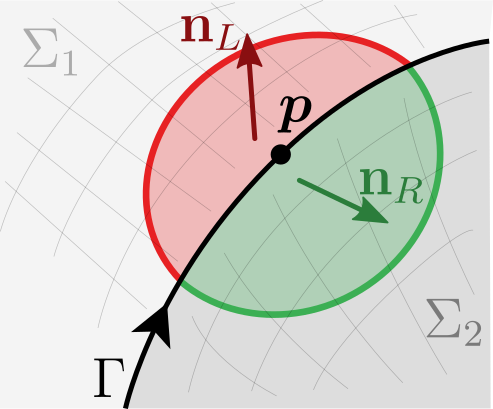
\includegraphics[width=5cm]{voisinage_courbe_singuliere.png}
%    \caption{Voisinage d'un point sur une courbe singulière.}
%\end{figure}



\section{Observations}%/Motivations}
[Objectif : justifier en quoi la construction intermédiaire d'une \guillemets{EdS partielle} (sous-ensemble de l'EdS qui contient l'EdB) permet de simplifier la construction d'un modèle \brep\ de l'EdB en évitant de construire des éléments de l'EdS qui sont trivialement exclues de l'EdB]
\par
définitions : 
\begin{itemize}
	\item \textit{zone d'influence}\footnote{\label{note_vocabulaire_notation}vocabulaire et notation à préciser \ldots} de $H \subseteq \Sigma$ sur l'EdB  (lieu des points de tangence entre $\EdB{\Sigma}{\rho}$ et $\sphere[H][\rho]$)
	\[ \influEdB{H}{\rho} := \EdB{\Sigma}{\rho} \cap \sphere[H][\rho] \]
	\item \textit{EdS propre}\footref{note_vocabulaire_notation} de $H \subseteq \Sigma$ 
	\[ \EdSpropre{H}{\rho} := \closure{ {\EdS{H}{\rho} \setminus \EdS{\boundary{H}}{\rho}} } \]
\end{itemize}
arguments :
\begin{enumerate}
	\item on sait décrire l'EdB simplement de manière \textit{implicite} (\cf \autoref{section:principe_huygens}) mais on cherche à en construire une représentation \textit{explicite}
	\item en revanche, on peut décrire explicitement l'EdS de chaque carreau ($\to$ introduire système définissant l'EdS à 2 paramètres)
	\item il est plus commode de voir l'EdS d'un carreau comme (un sous-ensemble de) la réunion de 10 nouveaux carreaux (intérieur $\to 2$ , bords $\to 4$ et ``coins'' $\to 4$)
	\item si on procède ainsi pour chaque carreau qui décrit l'interface, on construit beaucoup de nouveaux carreaux qui sont redondants, voire même trivialement exclus de l'EdB
%	\item la zone d'influence sur l'EdB d'une courbe singulière concave est vide (preuve?) (\ie cette courbe ne contribue pas à l'EdB et peut donc être ignorée)
%	\item la zone d'influence sur l'EdB d'une courbe singulière convexe $\Gamma$ est incluse dans la portion de son EdS qui est tangente aux EdS des deux nappes adhérentes à $\Gamma$ (preuve?), on appelle cette portion \textit{pseudo-EdS}\footref{note_vocabulaire_notation} de $\Gamma$ et on la note $\pseudoEdS{\Gamma}{\rho}$
	\item La zone d'influence sur l'EdB d'une courbe $\Gamma \subset \Sigma$ adhérente aux nappes régulières $\Left{\Sigma}$ et $\Right{\Sigma}$ est incluse dans le lieu des points de tangence entre $\EdS{\Gamma}{\rho}$, $\EdS{\Left{\Sigma}}{\rho}$ et $\EdS{\Right{\Sigma}}{\rho}$ (on appelle ce lieu \textit{pseudo-EdS}\footref{note_vocabulaire_notation} de $\Gamma$ et on le note $\pseudoEdS{\Gamma}{\rho}$).
	\begin{proof}
		En posant\footnote{introduire ces notations dans la \autoref{section:principe_huygens}.}
		\[
			\implicitsphere(\bx, \p) := \normtwo{\bx - \p}^2 - \rho(\p)^2,
		\]
		et, pour $H \subseteq \Sigma$, 
		\[
			\implicitEdB{H}(\bx) := \min_{\p \in H} \implicitsphere(\bx, \p),
		\]
		on veut démontrer que 
		\[
			\influEdB{\Gamma}{\rho} \subseteq 
			\left\{
				\bx \in \complement{\Omega} \mid \implicitEdB{\Gamma}(\bx) = \implicitEdB{\Left{\Sigma}}(\bx) = \implicitEdB{\Right{\Sigma}}(\bx) = 0
			\right\}
			\subseteq \pseudoEdS{\Gamma}{\rho}.
		\]
		\par
		Puisque $\Gamma \subseteq \left( \closure{\Left{\Sigma}} \cap \closure{\Right{\Sigma}} \right)$, on a $\implicitEdB{\Gamma} \geq \implicitEdB{\Left{\Sigma}}$ et $\implicitEdB{\Gamma} \geq \implicitEdB{\Right{\Sigma}}$.\par
		Or, si $\bx \in \influEdB{\Gamma}{\rho}$ alors\footnote{car $\forall \bx \in \EdB{\Sigma}{\rho}, \implicitEdB{\Gamma}(\bx) \geq 0$ et $\forall \bx \in \sphere[\Gamma][\rho], \implicitEdB{\Gamma}(\bx) \leq 0$.} $\implicitEdB{\Gamma}(\bx) = 0$ et donc $\implicitEdB{\Left{\Sigma}}(\bx) \leq 0$ et $\implicitEdB{\Right{\Sigma}}(\bx) \leq 0$.\par
		Mais si $\implicitEdB{\Left{\Sigma}} < 0$ ou $\implicitEdB{\Right{\Sigma}} < 0$ alors\footnote{car $\forall H \subseteq \Sigma, \forall \bx \in \EdB{\Sigma}{\rho}, \implicitEdB{H}(\bx) \geq 0$.} $\bx \notin \EdB{\Sigma}{\rho}$ et donc $\bx \notin \influEdB{\Gamma}{\rho}$.\par
		Donc si $\bx \in \influEdB{\Gamma}{\rho}$ alors $\implicitEdB{\Left{\Sigma}}(\bx) = 0$ et $\implicitEdB{\Right{\Sigma}}(\bx) = 0$.
	\end{proof}
	
	\item Si $\Gamma$ est une courbe singulière concave de $\Sigma$ alors sa zone d'influence sur l'EdB est vide (\ie $\Gamma$ ne contribue pas à l'EdB et peut donc être ignorée).
	\begin{proof}
		On veut montrer que $\influEdB{\Gamma}{\rho} = \varnothing$ (piste : montrer que si $\Gamma$ est concave alors, pour $\bx \in \complement{\Omega}$, $\implicitEdB{\Gamma}(\bx) = 0 \Rightarrow \implicitEdB{\Left{\Sigma}}(\bx) < 0$ ou $\implicitEdB{\Right{\Sigma}}(\bx) < 0$)
	\end{proof}
	
	\item si toutes les courbes singulières adhérentes à un point singulier sont concaves alors la zone d'influence sur l'EdB de ce point est vide (preuve?) (\ie ce point ne contribue pas à l'EdB et peut donc être ignoré)
	\item si toutes les courbes singulières adhérentes à un point singulier $\p$ \textit{ne sont pas} concaves (ou bien que $\p$ n'est adhérent à aucune courbe singulière, \eg le sommet d'un cône) on dit que $\p$ est convexe et sa zone d'influence sur l'EdB est la portion de $\sphere[\p][\rho(\p)]$ qui est tangente aux EdS de toutes les courbes singulières adhérentes à $\p$ (preuve?), on appelle cette portion \textit{pseudo-EdS}\footref{note_vocabulaire_notation} de $\p$ et on la note $\pseudoEdS{\p}{\rho}$
	\item l'EdB est incluse dans la réunion
	\begin{itemize}
		\item des EdS propres des nappes régulières, qui sont elles-mêmes contenues dans la réunion des EdS propres des faces \brep
		\item des pseudo-EdS des courbes singulières convexes, qui sont elles-mêmes contenues dans la réunion des pseudo-EdS des arêtes \brep\ convexes
		\item des pseudo-EdS des points singuliers convexes, qui sont elles-mêmes contenues dans la réunion des pseudo-EdS des sommets \brep\ convexes
	\end{itemize}
	\item[$\Rightarrow$] on construit d'abord une telle réunion (que l'on appelle \textit{EdS partielle}\footref{note_vocabulaire_notation}) puis on en élimine les régions qui sont exclues de l'EdB (au passage on constitue les relations topologiques qui assurent la validité du modèle \brep)
\end{enumerate}



\setlength{\imagewidth}{50mm}%
\setlength{\imageheight}{\imagewidth}%
\begin{figure}
	\centering
%	\definecolor{colorContourEdSnappe0}{rgb}{1,0,0}
%	\definecolor{colorContourEdSnappe1}{rgb}{0,1,0}
%	\definecolor{colorContourEdSarete}{rgb}{0,0,1}
	\colorlet{colorContourEdSnappe0}{mycolor_2}
	\colorlet{colorContourEdSnappe1}{mycolor_3}
	\colorlet{colorContourEdSarete}{mycolor_1}
	\colorlet{colorInterieurEdSnappe0}{colorContourEdSnappe0}%!50!white}
	\colorlet{colorInterieurEdSnappe1}{colorContourEdSnappe1}%!50!white}
	\colorlet{colorInterieurarete}{colorContourEdSarete!30!white}
	\colorlet{colorPseudoEdSarete}{mycolor_4}%colorContourEdSarete!70!black}
	\begin{tikzpicture}[
		x = \imagewidth,
		y = \imageheight,
		styleEdS/.style = {
			thick, fill opacity=0.2
		},
		stylePseudoEdS/.style = {
			line width=1.1pt, colorPseudoEdSarete, line cap=round%, dash pattern=on 4pt off 3pt
		},
		styleNappe/.style = {
			draw=black, thick, line cap=round
		}
	]
		\begin{scope}
			%\clip (-1,-0.55) rectangle (1,0.8);
			\begin{scope}[blend group = overlay]
\draw[styleEdS, draw=colorContourEdSnappe0, fill=colorInterieurEdSnappe0] 
(1.0398871880695557, -0.05029176412270403) -- 
(1.0183167534800655, -0.0449025730216131) -- 
(0.9970249326809821, -0.03889063165462239) -- 
(0.9760087070839042, -0.03227375493086215) -- 
(0.9552635663797575, -0.025069985986572035) -- 
(0.9347833891410695, -0.017297348539330626) -- 
(0.9145603833626653, -0.008973612328943836) -- 
(0.8945850834066453, -0.00011607984793962633) -- 
(0.8748463978997224, 0.009258598781243438) -- 
(0.8553317017006214, 0.019134577567845562) -- 
(0.83602696412914, 0.029496929643137104) -- 
(0.816916905210558, 0.04033172390652845) -- 
(0.7979851716958212, 0.05162606350851576) -- 
(0.7792145250047978, 0.06336808792773979) -- 
(0.7605870339290941, 0.07554694172716503) -- 
(0.742084265838364, 0.08815271410883804) -- 
(0.7236874711762205, 0.10117635410812229) -- 
(0.7053777571313378, 0.11460956667949797) -- 
(0.68713624745879, 0.12844469504848804) -- 
(0.6689442264517612, 0.1426745945736954) -- 
(0.650783265984124, 0.1572925030243364) -- 
(0.6326353353336946, 0.1722919116818077) -- 
(0.6144828941409042, 0.18766644106904284) -- 
(0.5963089693558062, 0.20340972444626615) -- 
(0.5780972173844605, 0.21951530152848314) -- 
(0.5598319728767698, 0.2359765242139565) -- 
(0.5414982857190578, 0.2527864754915883) -- 
(0.5230819478253321, 0.26993790213828667) -- 
(0.5045695112809123, 0.28742316133741974) -- 
(0.4859482992996188, 0.3052341809521778) -- 
(0.4672064113277807, 0.3233624328735336) -- 
(0.4483327234793507, 0.34179891862769246) -- 
(0.4293168853280881, 0.36053416626560775) -- 
(0.4101493139242216, 0.37955823745850226) -- 
(0.3908211857508439, 0.3988607436785092) -- 
(0.3713244271940277, 0.4184308703424265) -- 
(0.35165170397301176, 0.4382574078293584) -- 
(0.33179640986407155, 0.4583287883406225) -- 
(0.3117526549541225, 0.4786331276446601) -- 
(0.291515253577205, 0.4991582708338544) -- 
(0.28440988145616547, 0.5063087863339162) -- 
(0.27710254029824977, 0.5132527729480235) -- 
(0.2695992307813853, 0.5199845283794992) -- 
(0.26190611450974904, 0.5264985246127) -- 
(0.25402950895395104, 0.5327894124525396) -- 
(0.24597588226322395, 0.5388520259171669) -- 
(0.23775184795387602, 0.5446813864801907) -- 
(0.2293641594783722, 0.5502727071589723) -- 
(0.22081970467950082, 0.5556213964456214) -- 
(0.2121255001341817, 0.5607230620774737) -- 
(0.20328868539155925, 0.5655735146439503) -- 
(0.19431651711011275, 0.5701687710268386) -- 
(0.18521636309859835, 0.5745050576711679) -- 
(0.17599569626571607, 0.5785788136839961) -- 
(0.1666620884834703, 0.5823866937585616) -- 
(0.1572232043692633, 0.5859255709213973) -- 
(0.147686794991827, 0.5891925391001548) -- 
(0.13806069150616307, 0.592184915510027) -- 
(0.1283527987227171, 0.59490024285681) -- 
(0.1185710886160675, 0.597336291354796) -- 
(0.10872359377846114, 0.5994910605578396) -- 
(0.09881840082356977, 0.6013627810020942) -- 
(0.0888636437458856, 0.6029499156590681) -- 
(0.07886749724120823, 0.6042511611978101) -- 
(0.06883816999370787, 0.6052654490551841) -- 
(0.058783897935078405, 0.6059919463133578) -- 
(0.048712937481315166, 0.606430056383782) -- 
(0.038633558752670744, 0.6065794194970995) -- 
(0.028554038782357544, 0.6064399129985829) -- 
(0.018482654719573693, 0.6060116514488569) -- 
(0.008427677032433106, 0.6052949865298223) -- 
(-0.0016026372836175917, 0.6042905067558604) -- 
(-0.011600051486318735, 0.602999036990554) -- 
(-0.02155635585048546, 0.601421637769322) -- 
(-0.031463374409710254, 0.5995596044285232) -- 
(-0.04131297167034209, 0.5974144660417463) -- 
(-0.051097059292231184, 0.5949879841641577) -- 
(-0.06080760273075139, 0.592282151385939) -- 
(-0.07043662783464624, 0.5892991896960018) -- 
(-0.07997622739428173, 0.5860415486573246) -- 
(-0.08941856763492664, 0.5825119033954085) -- 
(-0.09875589464973036, 0.5787131524015046) -- 
(-0.10798054076711328, 0.5746484151524166) -- 
(-0.11708493084734278, 0.5703210295488347) -- 
(-0.12606158850312335, 0.5657345491743005) -- 
(-0.1349031422390926, 0.5608927403770597) -- 
(-0.14360233150518156, 0.5557995791771925) -- 
(-0.15215201265886868, 0.550459248001567) -- 
(-0.16054516483143072, 0.5448761322492933) -- 
(-0.16877489569337395, 0.5390548166905) -- 
(-0.17683444711431084, 0.5330000817013907) -- 
(-0.18471720071263423, 0.526716899338671) -- 
(-0.19241668329043216, 0.5202104292565717) -- 
(-0.19992657214918022, 0.5134860144698171) -- 
(-0.2072407002818455, 0.5065491769660245) -- 
(-0.2143530614371397, 0.49940561317112975) -- 
(-0.22125781505176162, 0.4920611892715692) -- 
(-0.22794929104657935, 0.48452193639705643) -- 
(-0.23442199448281317, 0.4767940456679094) -- 
(-0.24067061007439672, 0.4688838631109964) -- 
(-0.24669000655280857, 0.4607978844484749) -- 
(-0.252475240880793, 0.45254274976360276) -- 
(-0.25802156231150697, 0.44412523804800214) -- 
(-0.2633244162897616, 0.43555226163485494) -- 
(-0.2683794481921539, 0.42683086052259867) -- 
(-0.2731825069030178, 0.4179681965937866) -- 
(-0.2777296482232569, 0.4089715477338585) -- 
(-0.2820171381092618, 0.39984830185465114) -- 
(-0.2860414557392498, 0.39060595082755645) -- 
(-0.28979929640451024, 0.38125208433131086) -- 
(-0.2932875742231817, 0.3717943836194658) -- 
(-0.2965034246743312, 0.3622406152126584) -- 
(-0.29944420695025553, 0.35259862452086255) -- 
(-0.3021075061250724, 0.3428763294008567) -- 
(-0.30449113513782133, 0.3330817136542001) -- 
(-0.30659313658844445, 0.3232228204710559) -- 
(-0.3084117843451744, 0.31330774582524457) -- 
(-0.30994558496200736, 0.30334463182595317) -- 
(-0.31119327890509796, 0.29334166003155904) -- 
(-0.31215384158707016, 0.2833070447310568) -- 
(-0.312826484208392, 0.2732490261986096) -- 
(-0.3132106544051267, 0.2631758639267602) -- 
(-0.3133060367025248, 0.2530958298438609) -- 
(-0.31311255277408784, 0.24301720152129108) -- 
(-0.3126303615058885, 0.23294825537604125) -- 
(-0.311859858866096, 0.22289725987424416) -- 
(-0.31080167757981286, 0.21287246874123647) -- 
(-0.3094566866094909, 0.20288211418372343) -- 
(-0.30782599044135184, 0.19293440012961588) -- 
(-0.3059109281784007, 0.18303749549108922) -- 
(-0.30371307244077433, 0.1731995274563957) -- 
(-0.3012342280743293, 0.16342857481594059) -- 
(-0.29847643066853036, 0.15373266132810265) -- 
(-0.2954419448848546, 0.14411974913024406) -- 
(-0.29213326259708616, 0.13459773220032423) -- 
(-0.28855310084502717, 0.12517442987448518) -- 
(-0.2847043996033055, 0.11585758042593017) -- 
(-0.2805903193671125, 0.10665483471037143) -- 
(-0.27621423855685184, 0.09757374988326305) -- 
(-0.2715797507438321, 0.08862178319397956) -- 
(-0.26669066169928013, 0.07980628586203543) -- 
(-0.26155098626909984, 0.07113449704037526) -- 
(-0.25616494507694093, 0.0626135378706904) -- 
(-0.2505369610582869, 0.0542504056356455) -- 
(-0.2446716558284075, 0.0460519680128164) -- 
(-0.23857384588715833, 0.03802495743505638) -- 
(-0.23224853866374337, 0.030175965561924676) -- 
(-0.2257009284046912, 0.022511437866715802) -- 
(-0.218936391908417, 0.015037668343533813) -- 
(-0.2119604841098781, 0.0077607943387599816) -- 
(-0.20477893351894494, 0.0006867915111568382) -- 
(-0.19739763751623587, -0.006178531075252337) -- 
(-0.18982265751027697, -0.0128295357214991) -- 
(-0.18206021395996608, -0.019260760723262417) -- 
(-0.17411668126642477, -0.025466924855938287) -- 
(-0.1659985825384379, -0.0314429317115007) -- 
(-0.13814675776047186, -0.051389728187050454) -- 
(-0.11010149732607256, -0.07084782564879044) -- 
(-0.08187628874232598, -0.08980691529833429) -- 
(-0.05348514223118164, -0.10825785303989452) -- 
(-0.024942488161001697, -0.1261927311153278) -- 
(0.0037369331581589837, -0.14360494415097552) -- 
(0.032538188799990014, -0.16048924853161478) -- 
(0.0614462769517472, -0.17684181400939064) -- 
(0.09044625611895998, -0.19266026647310083) -- 
(0.11952337865593937, -0.20794372084870297) -- 
(0.14866322725437772, -0.22269280317764836) -- 
(0.17785185281340019, -0.23690966102675073) -- 
(0.2070759119251168, -0.25059796152153513) -- 
(0.2363228020507566, -0.26376287646259583) -- 
(0.265580792345058, -0.2764110541778851) -- 
(0.29483914802179645, -0.2885505779777789) -- 
(0.32408824615147613, -0.30019091130722525) -- 
(0.35331968085209736, -0.3113428299218043) -- 
(0.38252635598214596, -0.32201834164250964) -- 
(0.4117025636751192, -0.33223059445727054) -- 
(0.4408440473670057, -0.3419937739254134) -- 
(0.46994804835801024, -0.3513229909948436) -- 
(0.49901333540890813, -0.3602341614525258) -- 
(0.5280402173876334, -0.36874387829068567) -- 
(0.5570305395358062, -0.37686927828051764) -- 
(0.58598766449683, -0.38462790400140734) -- 
(0.6149164398129897, -0.39203756247917254) -- 
(0.6438231541327407, -0.39911618144689354) -- 
(0.6727154848442609, -0.40588166406421605) -- 
(0.7016024402409139, -0.41235174272506525) -- 
(0.7304942996033684, -0.4185438323598505) -- 
(0.7594025547290846, -0.4244748834068749) -- 
(0.788339856433129, -0.4301612343982981) -- 
(0.8173199693690699, -0.43561846388665537) -- 
(0.8463577381635287, -0.44086124123470705) -- 
(0.8754690673157085, -0.44590317560849646) -- 
(0.9046709165817106, -0.4507566623537582) -- 
(0.9339813126454302, -0.4554327258016044) -- 
(0.9634193767817649, -0.4599408574440896) -- 
(0.9693155652265435, -0.4609052976013954) -- 
(0.9752369803674806, -0.4617002980555111) -- 
(0.9811787540119019, -0.4623252052100757) -- 
(0.9871360012297284, -0.462779505308097) -- 
(0.9931038243695415, -0.46306282485432837) -- 
(0.9990773170851042, -0.4631749309223312) -- 
(1.0050515683690329, -0.463115731345972) -- 
(1.0110216665902994, -0.4628852747951948) -- 
(1.0169827035322463, -0.46248375073600834) -- 
(1.022929778427797, -0.46191148927471937) -- 
(1.0288580019885372, -0.46116896088654163) -- 
(1.0347625004243635, -0.4602567760288024) -- 
(1.0406384194503882, -0.45917568463906483) -- 
(1.0464809282778087, -0.45792657551857996) -- 
(1.0522852235854594, -0.45651047560157293) -- 
(1.0580465334687832, -0.45492854911096664) -- 
(1.0637601213629715, -0.453182096601235) -- 
(1.0694212899370539, -0.4512725538891737) -- 
(1.0750253849557292, -0.4492014908734677) -- 
(1.0805677991057672, -0.4469706102440253) -- 
(1.0860439757838356, -0.4445817460821393) -- 
(1.0914494128426344, -0.4420368623526284) -- 
(1.0967796662922613, -0.439338051289196) -- 
(1.1020303539537641, -0.4364875316743353) -- 
(1.1071971590618763, -0.43348764701519416) -- 
(1.1122758338139729, -0.4303408636168996) -- 
(1.1172622028623307, -0.42704976855492677) -- 
(1.1221521667468217, -0.42361706754817735) -- 
(1.1269417052652146, -0.4200455827345184) -- 
(1.1316268807783172, -0.41633825035060845) -- 
(1.1362038414472417, -0.41249811831791966) -- 
(1.1406688244001288, -0.4085283437369402) -- 
(1.1450181588257307, -0.40443219029161614) -- 
(1.1492482689913066, -0.40021302556616906) -- 
(1.153355677182352, -0.3958743182764921) -- 
(1.1573370065617445, -0.3914196354184033) -- 
(1.161188983945953, -0.3868526393350996) -- 
(1.1649084424960312, -0.3821770847062224) -- 
(1.1684923243211818, -0.37739681546101034) -- 
(1.1719376829927497, -0.372515761618077) -- 
(1.1752416859665806, -0.36753793605441143) -- 
(1.1784016169117477, -0.3624674312062588) -- 
(1.18141487794374, -0.35730841570459176) -- 
(1.1842789917602683, -0.3520651309479401) -- 
(1.186991603677939, -0.346741887615396) -- 
(1.1895504835681168, -0.3413430621226607) -- 
(1.1919535276903879, -0.33587309302404755) -- 
(1.1941987604221163, -0.33033647736339883) -- 
(1.196284335882667, -0.32473776697691586) -- 
(1.1982085394509678, -0.31908156475094274) -- 
(1.1999697891751553, -0.3133725208377806) -- 
(1.2015666370731508, -0.30761532883264203) -- 
(1.202997770323094, -0.30181472191489017) -- 
(1.2042620123426586, -0.2959754689567343) -- 
(1.2053583237563583, -0.2901023706025812) -- 
(1.206285803250054, -0.2842002553222653) -- 
(1.207043688311952, -0.27827397544140275) -- 
(1.2076313558594922, -0.272328403152133) -- 
(1.2080483227516046, -0.2663684265075271) -- 
(1.2082942461859139, -0.2603989454029569) -- 
(1.2083689239805722, -0.25442486754772686) -- 
(1.2082722947404756, -0.24845110443028384) -- 
(1.2080044379077421, -0.24248256728031795) -- 
(1.2075655736963986, -0.2365241630310776) -- 
(1.206956062911335, -0.2305807902852156) -- 
(1.2061764066516745, -0.22465733528748522) -- 
(1.2052272458988051, -0.2187586679075953) -- 
(1.2041093609894056, -0.21288963763652835) -- 
(1.2028236709739044, -0.20705506959961203) -- 
(1.2013712328609003, -0.20125976058962325) -- 
(1.1997532407481573, -0.19550847512318478) -- 
(1.1979710248408986, -0.18980594152369779) -- 
(1.1960260503582012, -0.18415684803402882) -- 
(1.1939199163283891, -0.17856583896215006) -- 
(1.1916543542744191, -0.1730375108628982) -- 
(1.1892312267903393, -0.16757640875899452) -- 
(1.186652526009987, -0.1621870224044293) -- 
(1.1839203719691895, -0.15687378259328583) -- 
(1.1810370108628132, -0.15164105751703733) -- 
(1.1780048131980896, -0.14649314917331077) -- 
(1.1748262718457447, -0.14143428982907139) -- 
(1.1715039999905257, -0.13646863854113506) -- 
(1.1680407289828147, -0.13160027773686905) -- 
(1.164439306093095, -0.12683320985789287) -- 
(1.1607026921711152, -0.12217135406953673) -- 
(1.156833959211675, -0.11761854303876616) -- 
(1.1528362878290375, -0.11317851978321818) -- 
(1.1487129646420393, -0.10885493459394213) -- 
(1.1444673795720515, -0.10465134203437362) -- 
(1.1401030230560127, -0.1005711980180092) -- 
(1.1356234831768246, -0.09661785696718544) -- 
(1.1310324427134695, -0.09279456905529601) -- 
(1.1263336761132745, -0.08910447753471601) -- 
(1.1215310463888133, -0.08555061615262943) -- 
(1.1166285019419941, -0.0821359066568845) -- 
(1.1116300733179485, -0.07886315639392778) -- 
(1.1065398698913833, -0.0757350560007904) -- 
(1.1013620764881287, -0.07275417719302638) -- 
(1.0961009499446528, -0.06992297065041925) -- 
(1.090760815608376, -0.06724376400219671) -- 
(1.0853460637816557, -0.06471875991340899) -- 
(1.0798611461123757, -0.06235003427404442) -- 
(1.0743105719340957, -0.060139534492371444) -- 
(1.0686989045587796, -0.058089077893909054) -- 
(1.0630307575251439, -0.05620035022734317) -- 
(1.057310790805714, -0.05447490427861628) -- 
(1.0515437069757052, -0.052914158594330525) -- 
(1.0457342473468798, -0.05151939631551329) -- 
cycle; 
\coordinate (EdS0) at (0.5780972173844605, 0.21951530152848314);
\draw[styleEdS, draw=colorContourEdSnappe1, fill=colorInterieurEdSnappe1] 
(-0.15169069257764084, 0.5507561630088252) -- 
(-0.17504146443852367, 0.5360596714869722) -- 
(-0.1980509650850808, 0.521674771969309) -- 
(-0.22073415534445154, 0.5076006935349764) -- 
(-0.24310719678293558, 0.49383615486428445) -- 
(-0.2651874165214464, 0.48037937081071636) -- 
(-0.2869932690927314, 0.46722807665123334) -- 
(-0.3085442956789244, 0.4543795691229797) -- 
(-0.32986108091481187, 0.44183076319743253) -- 
(-0.35096520730549785, 0.42957826339985106) -- 
(-0.37187920718936585, 0.41761844835234146) -- 
(-0.3926265120789917, 0.40594756710319946) -- 
(-0.4132313991330905, 0.39456184570400504) -- 
(-0.4337189344495226, 0.3834576024096734) -- 
(-0.45411491281992367, 0.3726313698053583) -- 
(-0.47444579354746064, 0.3620800221069333) -- 
(-0.49473863189786793, 0.35180090583672363) -- 
(-0.5150210057287882, 0.34179197203978184) -- 
(-0.5353209368240557, 0.33205190817334773) -- 
(-0.5556668064512493, 0.3225802677669589) -- 
(-0.5760872646692548, 0.313377595905848) -- 
(-0.5966111329481912, 0.3044455485284712) -- 
(-0.6172672997411849, 0.29578700344381215) -- 
(-0.6380846087839275, 0.2874061608610278) -- 
(-0.6590917401143961, 0.27930863108194903) -- 
(-0.6803170841236117, 0.2715015068394799) -- 
(-0.7017886093907949, 0.2639934175814647) -- 
(-0.7235337256421194, 0.25679456281626867) -- 
(-0.7455791439158018, 0.24991672147641975) -- 
(-0.7679507369237274, 0.2433732341503716) -- 
(-0.790673403666179, 0.23717895501566963) -- 
(-0.8137709435620123, 0.23135017041918954) -- 
(-0.837265946664578, 0.22590448133181817) -- 
(-0.8611797078861451, 0.22086064739230282) -- 
(-0.8855321744698602, 0.21623839097508424) -- 
(-0.9103419371234759, 0.21205816068103941) -- 
(-0.9356262761334505, 0.20834085484647802) -- 
(-0.961401274258467, 0.20510750705228062) -- 
(-0.9876820080846747, 0.20237893711210087) -- 
(-1.0144828286234011, 0.20017537250377648) -- 
(-1.0212111055321056, 0.19966127297052094) -- 
(-1.0279217854342695, 0.19895361221776484) -- 
(-1.034609301063352, 0.19805297732998992) -- 
(-1.041268104370191, 0.1969601154855073) -- 
(-1.0478926711257381, 0.19567593333658903) -- 
(-1.0544775055040283, 0.194201496257298) -- 
(-1.0610171446415886, 0.19253802745963902) -- 
(-1.0675061631695015, 0.19068690697876728) -- 
(-1.0739391777143585, 0.18864967052809295) -- 
(-1.080310851364378, 0.18642800822523345) -- 
(-1.086615898096975, 0.18402376318987038) -- 
(-1.092849087164114, 0.18143893001467354) -- 
(-1.0990052474318048, 0.1786756531105611) -- 
(-1.105079271670143, 0.17573622492766872) -- 
(-1.1110661207903312, 0.17262308405350335) -- 
(-1.116960828025175, 0.1693388131898597) -- 
(-1.122758503049575, 0.16588613701017735) -- 
(-1.1284543360376047, 0.1622679198991166) -- 
(-1.134043601652803, 0.15848716357622827) -- 
(-1.1395216629683755, 0.15454700460568818) -- 
(-1.1448839753140478, 0.1504507117941632) -- 
(-1.1501260900463823, 0.146201683478967) -- 
(-1.1552436582394316, 0.14180344470875594) -- 
(-1.1602324342926624, 0.13725964431910287) -- 
(-1.1650882794531596, 0.13257405190537624) -- 
(-1.1698071652491915, 0.12775055469543542) -- 
(-1.1743851768322795, 0.12279315432473595) -- 
(-1.1788185162250082, 0.11770596351652171) -- 
(-1.1831035054718757, 0.11249320266985613) -- 
(-1.1872365896905732, 0.10715919635832517) -- 
(-1.1912143400211617, 0.1017083697423152) -- 
(-1.195033456470697, 0.09614524489784283) -- 
(-1.1986907706509484, 0.09047443706498239) -- 
(-1.2021832484069326, 0.08470065081900341) -- 
(-1.2055079923340877, 0.07882867616739407) -- 
(-1.2086622441819999, 0.07286338457600965) -- 
(-1.2116433871426804, 0.06680972492764123) -- 
(-1.2144489480215048, 0.06067271941635902) -- 
(-1.2170765992890076, 0.054457459381035425) -- 
(-1.2195241610118286, 0.048169101081504476) -- 
(-1.2217896026612163, 0.04181286142086249) -- 
(-1.223871044797579, 0.03539401361745781) -- 
(-1.225766760629692, 0.028917882830160894) -- 
(-1.2274751774472679, 0.022389841740544255) -- 
(-1.228994877925694, 0.01581530609563598) -- 
(-1.2303246013018665, 0.00919973021494658) -- 
(-1.2314632444201337, 0.002548602465495202) -- 
(-1.2324098626474882, -0.004132559291410428) -- 
(-1.2331636706572482, -0.010838212277863062) -- 
(-1.2337240430805723, -0.017562793397715527) -- 
(-1.2340905150252757, -0.024300723851797427) -- 
(-1.2342627824615098, -0.03104641376615843) -- 
(-1.2342407024739888, -0.03779426682950015) -- 
(-1.2340242933805552, -0.04453868493594776) -- 
(-1.2336137347169822, -0.05127407282931096) -- 
(-1.2330093670880287, -0.05799484274498075) -- 
(-1.2322116918848693, -0.06469541904561071) -- 
(-1.2312213708691342, -0.07137024284673765) -- 
(-1.2300392256239019, -0.0780137766285043) -- 
(-1.2286662368721049, -0.08462050882965623) -- 
(-1.2271035436629079, -0.09118495842000482) -- 
(-1.2253524424267392, -0.09770167944756064) -- 
(-1.2234143858997542, -0.10416526555656458) -- 
(-1.2212909819186275, -0.11057035447267138) -- 
(-1.2189839920866703, -0.11691163245156061) -- 
(-1.2164953303123824, -0.1231838386872879) -- 
(-1.213827061221648, -0.12938176967671738) -- 
(-1.2109813984448963, -0.13550028353641472) -- 
(-1.2079607027806447, -0.14153430426842012) -- 
(-1.2047674802369503, -0.14747882597136147) -- 
(-1.201404379952393, -0.15332891699341478) -- 
(-1.1978741919983158, -0.15907972402366605) -- 
(-1.1941798450641463, -0.1647264761184806) -- 
(-1.1903244040277179, -0.17026448865953914) -- 
(-1.1863110674126072, -0.17568916724025793) -- 
(-1.182143164734598, -0.18099601147736766) -- 
(-1.1778241537394727, -0.1861806187444887) -- 
(-1.1733576175344205, -0.1912386878246079) -- 
(-1.1687472616154468, -0.19616602247842244) -- 
(-1.1639969107932449, -0.20095853492559496) -- 
(-1.1591105060200841, -0.2056122492360284) -- 
(-1.154092101120346, -0.2101233046283487) -- 
(-1.1489458594274173, -0.21448795867285936) -- 
(-1.1436760503297374, -0.21870259039630863) -- 
(-1.1382870457288554, -0.22276370328589631) -- 
(-1.1327833164124483, -0.22666792819002524) -- 
(-1.1271694283452947, -0.23041202611339306) -- 
(-1.1214500388812925, -0.23399289090410488) -- 
(-1.1156298928996586, -0.23740755183057632) -- 
(-1.1097138188685158, -0.2406531760460909) -- 
(-1.1037067248391326, -0.2437270709389667) -- 
(-1.0976135943741416, -0.24662668636638074) -- 
(-1.0914394824131113, -0.24934961677000123) -- 
(-1.085189511078903, -0.2518936031716694) -- 
(-1.0788688654282916, -0.2542565350474768) -- 
(-1.072482789150376, -0.2564364520786833) -- 
(-1.0660365802163472, -0.25843154577802285) -- 
(-1.059535586484222, -0.26024016099004743) -- 
(-1.052985201262192, -0.261860797264266) -- 
(-1.0463908588342665, -0.26329211009993686) -- 
(-1.0397580299519174, -0.2645329120614833) -- 
(-1.0330922172954773, -0.26558217376360543) -- 
(-1.0263989509090414, -0.2664390247252709) -- 
(-1.0196837836126742, -0.26710275409187817) -- 
(-1.0129522863957163, -0.2675728112249897) -- 
(-1.0062100437950219, -0.2678488061591494) -- 
(-0.9994626492619538, -0.2679305099254024) -- 
(-0.9927157005219838, -0.2678178547412513) -- 
(-0.9618600215907757, -0.26718218439906705) -- 
(-0.9312831146272719, -0.2666713947766457) -- 
(-0.9009530059793759, -0.26625843546062694) -- 
(-0.8708379447198517, -0.2659148207309584) -- 
(-0.8409063796084735, -0.26561086314225923) -- 
(-0.8111270158339738, -0.2653158722753026) -- 
(-0.781468939498758, -0.2649983223125783) -- 
(-0.7519017969860202, -0.26462599327495656) -- 
(-0.7223960161469252, -0.26416609165852906) -- 
(-0.6929230564929207, -0.2635853567615401) -- 
(-0.6634556761362759, -0.26285015915721244) -- 
(-0.6339682039861398, -0.26192659754746617) -- 
(-0.6044368066058047, -0.2607805996498903) -- 
(-0.5748397401256944, -0.2593780318721067) -- 
(-0.5451575786645209, -0.25768482137646576) -- 
(-0.5153734118323504, -0.2556670928082199) -- 
(-0.48547300507696894, -0.25329132053369574) -- 
(-0.4554449178937359, -0.25052449579649216) -- 
(-0.4252805762499636, -0.24733430683318938) -- 
(-0.3949742969699929, -0.24368932877385877) -- 
(-0.36452326326741585, -0.23955921915536818) -- 
(-0.33392745206468954, -0.23491491415179303) -- 
(-0.30318951516469345, -0.2297288202133098) -- 
(-0.2723146176820055, -0.2239749957199047) -- 
(-0.241310238347933, -0.21762931749468523) -- 
(-0.21018593731769367, -0.2106696275580442) -- 
(-0.17895309788205088, -0.203075856293629) -- 
(-0.14762464898207767, -0.1948301191796247) -- 
(-0.1162147756228702, -0.18591678534310513) -- 
(-0.0847386241761405, -0.17632251734497642) -- 
(-0.05321200916732435, -0.16603628272319448) -- 
(-0.02165112749206638, -0.1550493388439899) -- 
(0.009927714853966221, -0.14335519347778738) -- 
(0.041508359462259836, -0.130949544186216) -- 
(0.07307503265108445, -0.11783020005372988) -- 
(0.1046125612256801, -0.1039969895135833) -- 
(0.13610656612738772, -0.08945165801084692) -- 
(0.16754363425536342, -0.07419775903601292) -- 
(0.19891146963183234, -0.058240541683307556) -- 
(0.2078176233741046, -0.053513397115755326) -- 
(0.21658463702996975, -0.04853294113247408) -- 
(0.22520530776875866, -0.04330326559216415) -- 
(0.23367255299267653, -0.03782866710811363) -- 
(0.2419794161557458, -0.032113643518173626) -- 
(0.25011907247918735, -0.026162890189410426) -- 
(0.25808483455854336, -0.01998129616047086) -- 
(0.2658701578579365, -0.013573940124830638) -- 
(0.27346864608695, -0.006946086258225556) -- 
(0.2808740564557121, -0.00010317989369318381) -- 
(0.28808030480386737, 0.006949156952220904) -- 
(0.29508147059921985, 0.014205130198417112) -- 
(0.3018718018019427, 0.021658778459561226) -- 
(0.3084457195903571, 0.029303977943858264) -- 
(0.3147978229443984, 0.03713444748425651) -- 
(0.32092289308300304, 0.04514375369894848) -- 
(0.3268158977517707, 0.053325316276928963) -- 
(0.33247199535738053, 0.06167241338426771) -- 
(0.3378865389453618, 0.070178187186655) -- 
(0.34305508001795404, 0.07883564948368263) -- 
(0.34797337218891744, 0.08763768745023151) -- 
(0.3526373746722923, 0.09657706948024913) -- 
(0.3570432556022406, 0.10564645112811495) -- 
(0.36118739518124277, 0.11483838114271346) -- 
(0.3650663886540617, 0.12414530758925614) -- 
(0.36867704910503296, 0.13355958405382418) -- 
(0.3720164100763803, 0.1430734759255331) -- 
(0.3750817280054082, 0.15267916675115878) -- 
(0.3778704844785657, 0.16236876465700348) -- 
(0.38038038830053345, 0.17213430883272657) -- 
(0.3826093773766308, 0.18196777607181205) -- 
(0.3845556204069979, 0.1918610873632996) -- 
(0.38621751839116114, 0.2018061145293642) -- 
(0.38759370594174447, 0.2117946869032897) -- 
(0.3886830524062495, 0.221818598042351) -- 
(0.38948466279597954, 0.23186961247008944) -- 
(0.38999787852134793, 0.2419394724424407) -- 
(0.39022227793296416, 0.2520199047321589) -- 
(0.3901576766680531, 0.2621026274259604) -- 
(0.38980412780192564, 0.2721793567288041) -- 
(0.3891619218043716, 0.2822418137697178) -- 
(0.3882315863010155, 0.2922817314035794) -- 
(0.38701388563982797, 0.30229086100326336) -- 
(0.3855098202631504, 0.3122609792365748) -- 
(0.3837206258857481, 0.3221838948223994) -- 
(0.3816477724795685, 0.3320514552605226) -- 
(0.3792929630660361, 0.34185555352958685) -- 
(0.3766581323168795, 0.35158813474768247) -- 
(0.37374544496463746, 0.36124120279010385) -- 
(0.3705572940241511, 0.3708068268588306) -- 
(0.3670962988265031, 0.38027714799833723) -- 
(0.3633653028670198, 0.3896443855523788) -- 
(0.3593673714691029, 0.398900843556447) -- 
(0.35510578926581204, 0.40803891706064477) -- 
(0.35058405750126476, 0.4170510983777851) -- 
(0.3458058911540741, 0.42592998325158) -- 
(0.34077521588518467, 0.434668276939853) -- 
(0.33549616481261524, 0.4432588002077763) -- 
(0.3299730751157592, 0.4516944952262091) -- 
(0.32421048447203105, 0.45996843137029075) -- 
(0.3182131273287865, 0.46807381091352634) -- 
(0.31198593101358096, 0.47600397461268296) -- 
(0.3055340116859604, 0.4837524071789122) -- 
(0.29886267013410983, 0.49131274263060226) -- 
(0.2919773874198163, 0.49867876952356016) -- 
(0.2848838203753203, 0.5058444360542305) -- 
(0.2775877969557575, 0.5128038550317544) -- 
(0.27009531145100973, 0.5195513087147872) -- 
(0.26241251956089684, 0.5260812535090974) -- 
(0.2545457333377575, 0.5323883245220917) -- 
(0.24650141600057368, 0.5384673399705187) -- 
(0.23828617662489873, 0.5443133054377355) -- 
(0.22990676471295257, 0.5499214179770362) -- 
(0.2213700646483436, 0.5552870700576722) -- 
(0.21268309003997596, 0.5604058533503213) -- 
(0.2038529779597865, 0.5652735623488971) -- 
(0.194886983079046, 0.569886197825722) -- 
(0.1857924717080448, 0.5742399701172248) -- 
(0.1765769157440554, 0.5783313022374652) -- 
(0.16724788653254827, 0.5821568328169241) -- 
(0.1578130486467014, 0.5857134188641493) -- 
(0.14828015359031646, 0.5889981383479833) -- 
(0.1386570334293139, 0.5920082925982559) -- 
(0.1289515943570395, 0.594741408522965) -- 
(0.11917181019866954, 0.597195240640128) -- 
(0.10932571586004947, 0.599367772922632) -- 
(0.0994214007263517, 0.6012572204545673) -- 
(0.08946700201597302, 0.6028620308976845) -- 
(0.0794706980951321, 0.6041808857667695) -- 
(0.06944070175866277, 0.6052127015128886) -- 
(0.059385253482519385, 0.6059566304136137) -- 
(0.049312614653541476, 0.6064120612694976) -- 
(0.03923106078203639, 0.6065786199062245) -- 
(0.02914887470276048, 0.6064561694820254) -- 
(0.019074339769881793, 0.6060448106001051) -- 
(0.009015733051514832, 0.6053448812259884) -- 
(-0.0010186814705782643, 0.6043569564098533) -- 
(-0.011020659690536047, 0.6030818478140791) -- 
(-0.020981984151616465, 0.6015206030463986) -- 
(-0.030894470797520404, 0.5996745047992016) -- 
(-0.04074997569627459, 0.5975450697956954) -- 
(-0.050540401731149445, 0.5951340475437916) -- 
(-0.06025770525311238, 0.5924434188987395) -- 
(-0.06989390268935552, 0.5894753944356885) -- 
(-0.07944107710246415, 0.5862324126335174) -- 
(-0.08889138469483893, 0.5827171378714212) -- 
(-0.09823706125302803, 0.5789324582399011) -- 
(-0.10747042852667375, 0.5748814831679595) -- 
(-0.11658390053683444, 0.570567540868444) -- 
(-0.12556998980849549, 0.5659941756036453) -- 
(-0.13442131352215392, 0.5611651447733902) -- 
(-0.14313059957941804, 0.5560844158280247) -- 
cycle; 
\coordinate (EdS1) at (-0.4337189344495226, 0.3834576024096734);
\end{scope}
\draw[styleEdS, draw=colorContourEdSarete, fill=colorInterieurarete] (0.03846156134313788, 0.25480769814250004) circle (0.3464951869522779);
\draw[stylePseudoEdS] (0.29657632742188633, 0.5040452822876815) arc (43.99759375651435:122.72148004933781:0.3588071986713943) node[above, pos=0.5, inner sep=2pt] {$\pseudoEdS{\crete}{\rho}$};
\path[decoration={text along path, raise={1ex}, text color=colorContourEdSarete, text={{$\implicitEdB{\crete}$} {$=$} {$0$}{}}, text align={center}}, decorate] (-0.21027863798930502, 0.0060674988100571925) arc (225:310:0.3517717634033278);
\draw[
    styleNappe,
    postaction={
        decoration={
            text along path, raise={1ex}, text={{$\Right{\nappe}$}{}}, text align=center, reverse path
        },
        decorate
    }
]
(1.0, -0.2548076981425002) .. controls (0.6394231211989716, -0.18750003123338313) and (0.33205293517056217, 0.00165690420180032) .. (0.03846156134313788, 0.25480769814250004) node[pos=0.35, above] (labelNappe0) {};
\node[colorContourEdSnappe0, inner sep=0.15\imagewidth, below] at (labelNappe0) {$\implicitEdB{\Right{\nappe}} < 0$};
\path[decoration={text along path, raise={1ex}, text color=colorContourEdSnappe0, text={{$\implicitEdB{\Right{\nappe}}$} {$=$} {$0$}{}}, text align={center}}, decorate] 
(0.291515253577205, 0.4991582708338544) -- 
(0.3117526549541225, 0.4786331276446601) -- 
(0.33179640986407155, 0.4583287883406225) -- 
(0.35165170397301176, 0.4382574078293584) -- 
(0.3713244271940277, 0.4184308703424265) -- 
(0.3908211857508439, 0.3988607436785092) -- 
(0.4101493139242216, 0.37955823745850226) -- 
(0.4293168853280881, 0.36053416626560775) -- 
(0.4483327234793507, 0.34179891862769246) -- 
(0.4672064113277807, 0.3233624328735336) -- 
(0.4859482992996188, 0.3052341809521778) -- 
(0.5045695112809123, 0.28742316133741974) -- 
(0.5230819478253321, 0.26993790213828667) -- 
(0.5414982857190578, 0.2527864754915883) -- 
(0.5598319728767698, 0.2359765242139565) -- 
(0.5780972173844605, 0.21951530152848314) -- 
(0.5963089693558062, 0.20340972444626615) -- 
(0.6144828941409042, 0.18766644106904284) -- 
(0.6326353353336946, 0.1722919116818077) -- 
(0.650783265984124, 0.1572925030243364) -- 
(0.6689442264517612, 0.1426745945736954) -- 
(0.68713624745879, 0.12844469504848804) -- 
(0.7053777571313378, 0.11460956667949797) -- 
(0.7236874711762205, 0.10117635410812229) -- 
(0.742084265838364, 0.08815271410883804) -- 
(0.7605870339290941, 0.07554694172716503) -- 
(0.7792145250047978, 0.06336808792773979) -- 
(0.7979851716958212, 0.05162606350851576) -- 
(0.816916905210558, 0.04033172390652845) -- 
(0.83602696412914, 0.029496929643137104) -- 
(0.8553317017006214, 0.019134577567845562) -- 
(0.8748463978997224, 0.009258598781243438) -- 
(0.8945850834066453, -0.00011607984793962633) -- 
(0.9145603833626653, -0.008973612328943836) -- 
(0.9347833891410695, -0.017297348539330626) -- 
(0.9552635663797575, -0.025069985986572035) -- 
(0.9760087070839042, -0.03227375493086215) -- 
(0.9970249326809821, -0.03889063165462239) -- 
(1.0183167534800655, -0.0449025730216131) -- 
(1.0398871880695557, -0.05029176412270403);
\draw[
    styleNappe,
    postaction={
        decoration={
            text along path, raise={1ex}, text={{$\Left{\nappe}$}{}}, text align=center, reverse path
        },
        decorate
    }
]
(0.03846156134313788, 0.25480769814250004) .. controls (-0.28894796328001215, 0.06631655134905) and (-0.5865384951744124, -0.014423064681421358) .. (-0.9999999999999998, -0.0336538334545584) node[pos=0.65, above] (labelNappe1) {};
\node[colorContourEdSnappe1, inner sep=0.15\imagewidth, below] at (labelNappe1) {$\implicitEdB{\Left{\nappe}} < 0$};
\path[decoration={text along path, raise={1ex}, text color=colorContourEdSnappe1, text={{$\implicitEdB{\Left{\nappe}}$} {$=$} {$0$}{}}, text align={center}}, decorate] 
(-1.0144828286234011, 0.20017537250377648) -- 
(-0.9876820080846747, 0.20237893711210087) -- 
(-0.961401274258467, 0.20510750705228062) -- 
(-0.9356262761334505, 0.20834085484647802) -- 
(-0.9103419371234759, 0.21205816068103941) -- 
(-0.8855321744698602, 0.21623839097508424) -- 
(-0.8611797078861451, 0.22086064739230282) -- 
(-0.837265946664578, 0.22590448133181817) -- 
(-0.8137709435620123, 0.23135017041918954) -- 
(-0.790673403666179, 0.23717895501566963) -- 
(-0.7679507369237274, 0.2433732341503716) -- 
(-0.7455791439158018, 0.24991672147641975) -- 
(-0.7235337256421194, 0.25679456281626867) -- 
(-0.7017886093907949, 0.2639934175814647) -- 
(-0.6803170841236117, 0.2715015068394799) -- 
(-0.6590917401143961, 0.27930863108194903) -- 
(-0.6380846087839275, 0.2874061608610278) -- 
(-0.6172672997411849, 0.29578700344381215) -- 
(-0.5966111329481912, 0.3044455485284712) -- 
(-0.5760872646692548, 0.313377595905848) -- 
(-0.5556668064512493, 0.3225802677669589) -- 
(-0.5353209368240557, 0.33205190817334773) -- 
(-0.5150210057287882, 0.34179197203978184) -- 
(-0.49473863189786793, 0.35180090583672363) -- 
(-0.47444579354746064, 0.3620800221069333) -- 
(-0.45411491281992367, 0.3726313698053583) -- 
(-0.4337189344495226, 0.3834576024096734) -- 
(-0.4132313991330905, 0.39456184570400504) -- 
(-0.3926265120789917, 0.40594756710319946) -- 
(-0.37187920718936585, 0.41761844835234146) -- 
(-0.35096520730549785, 0.42957826339985106) -- 
(-0.32986108091481187, 0.44183076319743253) -- 
(-0.3085442956789244, 0.4543795691229797) -- 
(-0.2869932690927314, 0.46722807665123334) -- 
(-0.2651874165214464, 0.48037937081071636) -- 
(-0.24310719678293558, 0.49383615486428445) -- 
(-0.22073415534445154, 0.5076006935349764) -- 
(-0.1980509650850808, 0.521674771969309) -- 
(-0.17504146443852367, 0.5360596714869722) -- 
(-0.15169069257764084, 0.5507561630088252);
\coordinate (Gamma) at (0.03846156134313788, 0.25480769814250004);
\fill[black] (Gamma) circle (1.2pt);
\node[above] at (Gamma) {$\crete$};

			\node[colorContourEdSarete] at ([shift={(120:0.2\imagewidth)}]Gamma) {$\implicitEdB{\Gamma} < 0$};
		\end{scope}
	\end{tikzpicture}
	\caption{Vue en coupe \ldots}
\end{figure}







\section{Construction d'une EdS partielle}
\label{section:def_canal_surface}

[Objectif : donner les étapes de la construction d'une EdS partielle sous la forme d'un ensemble de carreaux restreints (paramétrisation + courbes de restriction du domaine paramétrique) avec des relations d'adjacences partielles)]




\subsection{Paramétrisation de l'EdS propre d'une face \brep}% carreau paramétrique restreint}
\label{section:parametrisation_eds_propre_face}
\def\indice{_0}
\def\carreau{\Sigma\indice}
\def\face{\brepface\indice}

\begin{enumerate}
	\item paramétrisation $\eos$ de l'EdS propre d'un carreau non-restreint $\carreau \colon (\left[\lo{u},\hi{u}\right] \times \left[\lo{v},\hi{v}\right], \bs)$
	\begin{enumerate}
		\item rappeler système définissant une EdS propre à 2 paramètres
		\begin{subequations}
			\label{eq:sys_envelope_of_spheres}
			\begin{empheq}[left={\empheqlbrace\,}]{align}
				\implicitsphere_{\rho}(\eos(u,v), \bs(u,v)) &= 0, \label{eq:sys_envelope_of_spheres_Sphere} \\%[\sysvspace]
				\frac{\partial }{\partial u}\implicitsphere_{\rho}(\eos(u,v), \bs(u,v)) &= 0, \label{eq:sys_envelope_of_spheres_PlaneU} \\%[\sysvspace]
				\frac{\partial }{\partial v}\implicitsphere_{\rho}(\eos(u,v), \bs(u,v)) &= 0. \label{eq:sys_envelope_of_spheres_PlaneV}
			\end{empheq}
		\end{subequations}				
		\item interprétation : intersection de cercles caractéristiques (voir figure \autoref{fig:EdS_propre_carreau}) $\to$ 2 points (\ie 2 nouveaux carreaux), on garde celui dans le sens de $+\unv$ (\ie $\EdSpropreplus{\carreau}{\rho}$, l'autre ($\EdSpropremoins{\carreau}{\rho}$) est trivialement exclu de l'EdB)
		\item paramétrisation à la Gelston \cite{gelston1995} : \\
		En considérant $\rho$ comme une fonction des paramètres $u$ et $v$, on peut réécrire le système \eqref{eq:sys_envelope_of_spheres} 
		\begin{subequations}
			%\label{eq:sys_envelope_of_spheres}
			\begin{empheq}[left={\empheqlbrace\,}]{align}
				\normtwo{\eos - \bs}^2 - \rho^2 &= 0, \\
				\dotprod{\left( \eos - \bs \right)}{\left( \eos_u - \bsu \right)} - \rho \rho_u &= 0,\\
				\dotprod{\left( \eos - \bs \right)}{\left( \eos_v - \bsv \right)} - \rho \rho_v &= 0.
			\end{empheq}
		\end{subequations}	
		%Or $\eos - \bs$ est orthogonal à la sphère $\sphere[\bs][\rho]$ et donc aussi à $\EdSpropre{\carreau}{\rho}$.
		Or $\eos - \bs$ est un rayon de la sphère $\sphere[\bs][\rho]$ et est donc orthogonal à $\EdSpropre{\carreau}{\rho}$ en $\eos$.
		Donc $\dotprod{\left( \eos - \bs \right)}{\eos_u} = \dotprod{\left( \eos - \bs \right)}{\eos_v} = 0$ et on a finalement
		\begin{subequations}
			%\label{eq:sys_envelope_of_spheres}
			\begin{empheq}[left={\empheqlbrace\,}]{align}
				\normtwo{\eos - \bs}^2 - \rho^2 &= 0, \\
				\dotprod{\left( \eos - \bs \right)}{\bsu} + \rho \rho_u &= 0,\\
				\dotprod{\left( \eos - \bs \right)}{\bsv} + \rho \rho_v &= 0.
			\end{empheq}
		\end{subequations}	
%		\begin{equation}
%		    \left\{\begin{matrix}
%		        \normtwo{\eos - \bs}^2 - \rho^2 &= 0, \\
%		        \dotprod{\left( \eos - \bs \right)}{\bsu} + \rho \rho_u &= 0, \\
%		        \dotprod{\left( \eos - \bs \right)}{\bsv} + \rho \rho_v &= 0.
%		    \end{matrix}\right.
%		\end{equation}
		On cherche alors une paramétrisation de la forme
		\begin{equation}
			\eos(u,v) = \bs(u,v) + \rho(u,v) \unv_{\envelope}(u,v),
		\end{equation}
		où $\unv_{\envelope}$ est la direction normale à $\EdSpropre{\carreau}{\rho}$, qui vérifie
		\begin{subequations}
			\begin{empheq}[left={\empheqlbrace\,}]{align}
				\normtwo{\unv_{\envelope}}       &= 1,        \\
				\dotprod{\unv_{\envelope}}{\bsu} &= -\rho_u , \\
				\dotprod{\unv_{\envelope}}{\bsv} &= -\rho_v .
			\end{empheq}
		\end{subequations}	
		On décompose $\unv_{\envelope} = \mathrm{n}_u \bsu + \mathrm{n}_v \bsv + \mathrm{n}_n \unv$, où $\unv = \unitized{\crossprod{\bsu}{\bsv}}$.\\
		Puisque $\dotprod{\bsu}{\unv} = \dotprod{\bsv}{\unv} = 0$, on a 
		\[
			\transpose{\jacobian{\bs}} \unv_{\envelope} = \fff_{\bs} \colvec{\mathrm{n}_u \\ \mathrm{n}_v} = -\colvec{\rho_u \\ \rho_v}.
		\]
		Si on pose $\bt = \jacobian{\bs} \colvec{\mathrm{n}_u \\ \mathrm{n}_v}$ (on a alors $\unv_{\envelope} = \bt + \mathrm{n}_n \unv$), on a
		\[
			\bt = - \jacobian{\bs} \inverse{ \left(\fff_{\bs}\right) } \colvec{\rho_u \\ \rho_v},
		\]
		soit
		\[
			\bt = \frac{
				\left( \rho_v I_{1,2} - \rho_u I_{2,2} \right) \bsu + 
				\left( \rho_u I_{1,2} - \rho_v I_{1,1} \right) \bsv
			}{
				\determinant{\fff_{\bs}}
			}.
		\]
		Si $\normtwo{\bt} \leq 1$ alors on a $\unv_{\envelope}^{\pm} = \bt \pm \sqrt{1 - \normtwo{\bt}^2} \unv$.
				
		\item différence avec le simple transport suivant la normale $\to$ abordé dans la \autoref{section:discretisation_EdS_propre_carreau}
	\end{enumerate}
	\item conservation du domaine paramétrique (pas de re-paramétrisation) $\Rightarrow$ coordonnées $(x,y,z)$ des courbes de restriction données directement par la nouvelle paramétrisation (voir \autoref{fig:EdS_propre_carreau_restreint}).
\end{enumerate}


\begin{figure}%[!htp]
	\centering
	\setlength{\imagewidth}{120mm}%
	\setlength{\imageheight}{0.625\imagewidth}%
	\DTLsetseparator{,}%
	\DTLloaddb[noheader,keys={x,y}]{dbsurfpoint}{figures/data/EdS_propre_carreau/surface_point.dat}%
	\DTLloaddb[noheader,keys={x,y}]{dbsurfvectors}{figures/data/EdS_propre_carreau/surface_vectors.dat}%
	\DTLloaddb[noheader,keys={x,y}]{dbEdSpoints}{figures/data/EdS_propre_carreau/envelope_points.dat}%
	\DTLloaddb[noheader,keys={x,y}]{dbEdSnormals}{figures/data/EdS_propre_carreau/envelope_normals.dat}%
	\begin{tikzpicture}[
		x = \imagewidth,
		y = \imageheight,
		point/.style = {circle, scale=0.27, fill=black},
		vector/.style = {-latex', thick},
		label/.style = {inner sep=2pt},
		txt/.style = {font=\small}
	]
		\node[anchor=south west, inner sep=0] at (0,0) {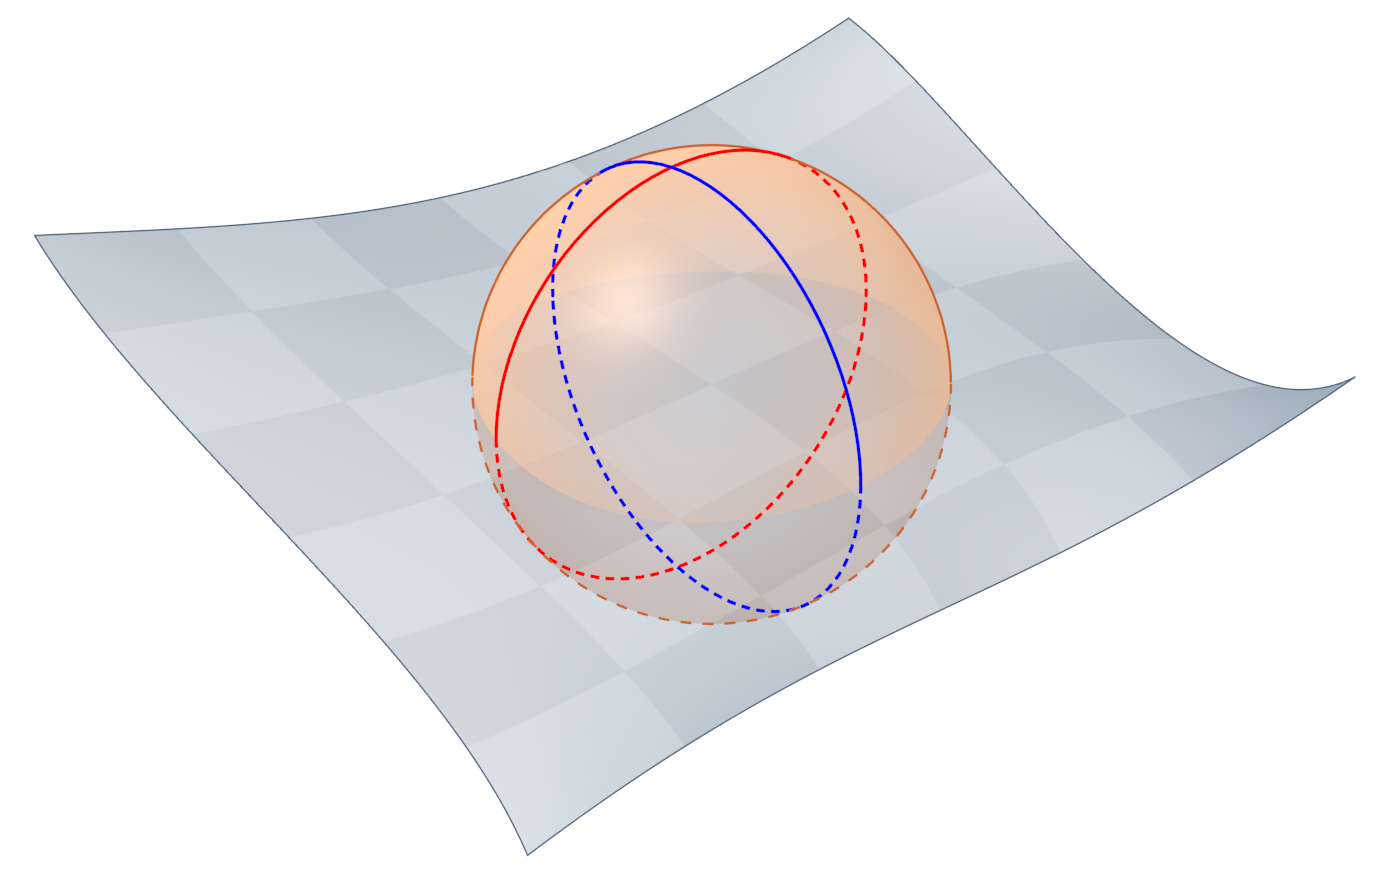
\includegraphics[width=\imagewidth]{figures/images/EdS_propre_carreau/EdS_propre_carreau.png}};
		%\drawGrid{10}{10}{black, thin, dotted}
		\DTLassign{dbsurfpoint}{1}{\spx=x, \spy=y}
		\coordinate (s) at (\spx, \spy);
		%
		\DTLassign{dbEdSpoints}{1}{\eppx=x, \eppy=y}
		\DTLassign{dbEdSpoints}{2}{\empx=x, \empy=y}
		\coordinate (ep) at (\eppx, \eppy);
		\coordinate (em) at (\empx, \empy);
		\node [anchor=north, txt, xshift=0pt, label] at (ep) {$\eos^+$};
		\node [anchor=south, txt, xshift=3pt, yshift=2pt, label] at (em) {$\eos^-$};
		%
		\DTLassign{dbsurfvectors}{1}{\sux=x, \suy=y}
		\coordinate (su) at (\sux, \suy);
		\draw [vector, red] (s) -- (su) node [below, xshift=-1pt, label, txt] {$\bsu$};
		%
		\DTLassign{dbsurfvectors}{2}{\svx=x, \svy=y}
		\coordinate (sv) at (\svx, \svy);
		\draw [vector, blue] (s) -- (sv) node [above, xshift=-5pt, label, txt] {$\bsv$};
		%
		\DTLassign{dbsurfvectors}{3}{\snx=x, \sny=y}
		\coordinate (sn) at (\snx, \sny);
		\draw [vector] (s) -- (sn) node [right, label, txt, black] {$\unv$};
		%
		\DTLassign{dbEdSnormals}{1}{\epnx=x, \epny=y}
		\coordinate (epn) at (\epnx, \epny);
		\node [anchor=west, label, txt, xshift=0pt] at (epn) {$\unv_{\envelope}^+$};
		\draw [dotted, thick, shorten >= 14pt] (s) -- (ep);
		\draw [vector] (ep) -- (epn);
		%
		\DTLassign{dbEdSnormals}{2}{\emnx=x, \emny=y}
		\coordinate (emn) at (\emnx, \emny);
		\node [anchor=west, label, txt, xshift=0pt] at (emn) {$\unv_{\envelope}^+$};
		\draw [dotted, thick, shorten <= 0pt, shorten >= 14pt] (s) -- (em);
		\draw [vector] (em) -- (emn);
		%
		\node [point] at (s) {};
		\node [point] at (ep) {};
		\node [point] at (em) {};
		%
		\node [anchor=east, txt, inner sep=2pt] at (s) {$\bs(u,v)$};
		\definecolor{colorSurfLabel}{rgb}{0.330, 0.413, 0.500}
		\node [txt, label, colorSurfLabel] at (0.1,0.68) {$\carreau$};
	\end{tikzpicture}
	\DTLgdeletedb{dbsurfpoint}%
	\DTLgdeletedb{dbsurfvectors}%
	\DTLgdeletedb{dbEdSpoints}%
	\DTLgdeletedb{dbEdSnormals}%
	\caption{Paramétrisation de l'EdS propre d'un carreau paramétrique.}
	\label{fig:EdS_propre_carreau}
\end{figure}

\begin{figure}
	\centering
	%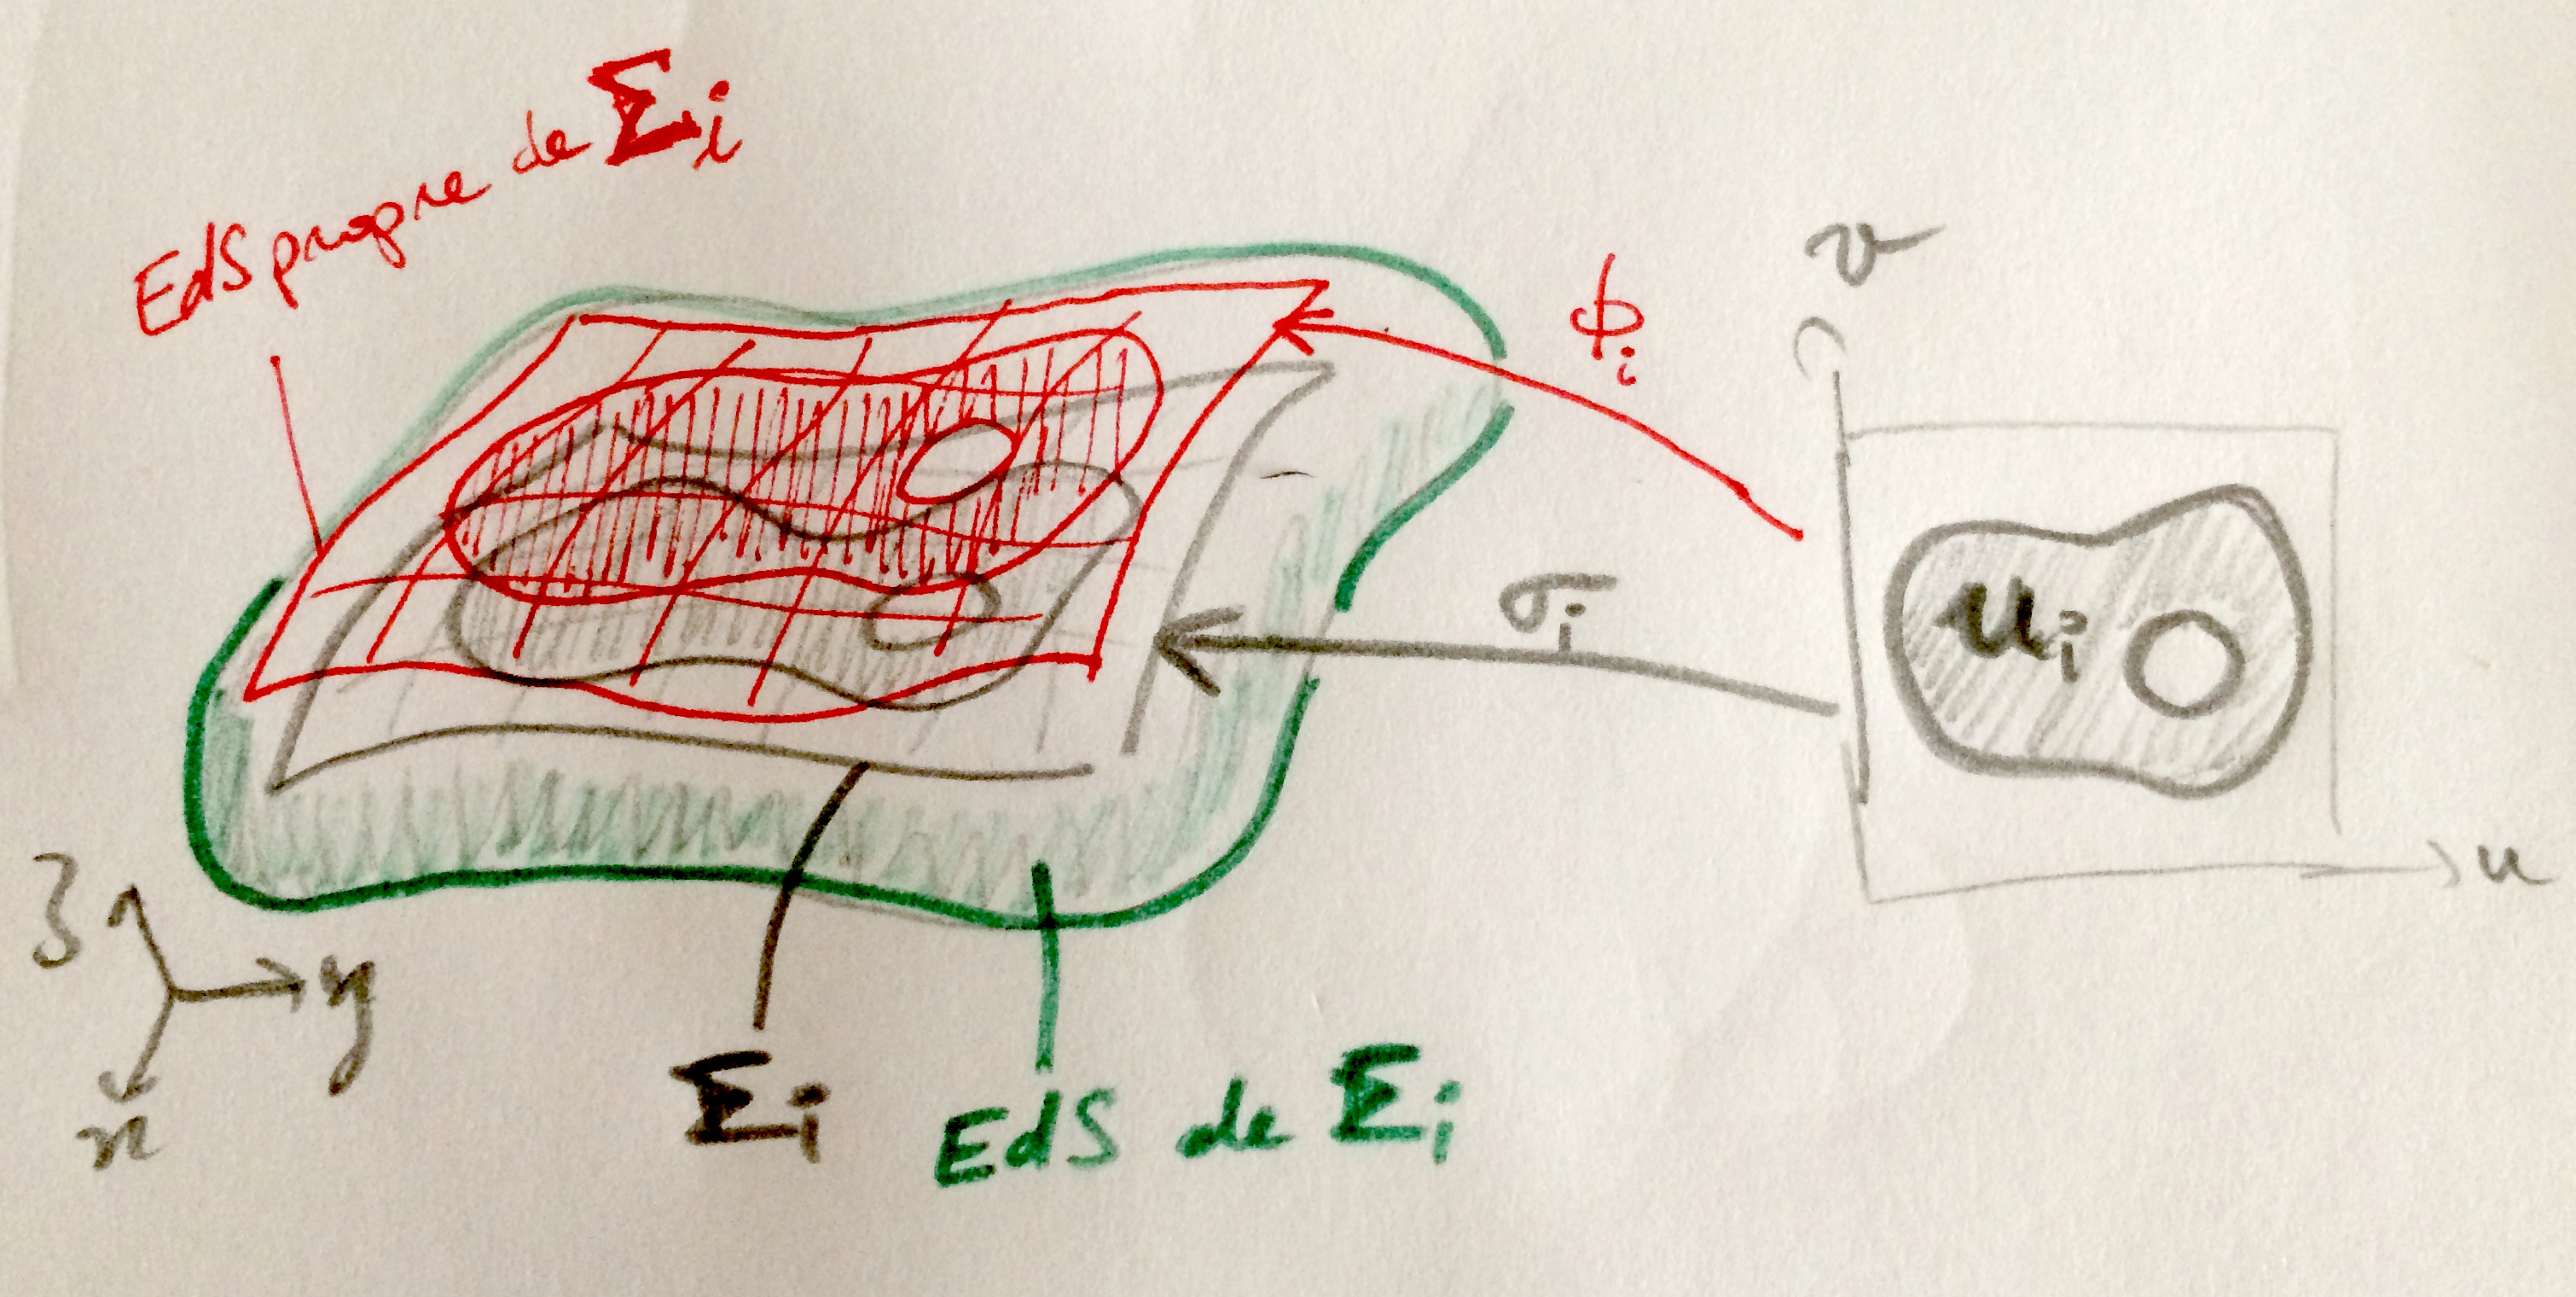
\includegraphics[width=10cm]{EdS_propre_carreau_restreint.JPG}
	\setlength{\imagewidth}{80mm}%
\setlength{\imageheight}{0.75\imagewidth}%
\definecolor{colorEdS}{HTML}{81BD3E}%
%\definecolor{colorInterieurDomaineUV}{HTML}{ADD9F4}%
%\definecolor{colorBordDomaineUV}{HTML}{6BA2BF}%
%\colorlet{colorInterieurDomaineUV}{mycolor_5}%
%\definecolor{colorInterieurDomaineUV}{RGB}{235, 220, 178}
\definecolor{colorInterieurDomaineUV}{HTML}{FFEED5}%
\colorlet{colorBordDomaineUV}{colorInterieurDomaineUV!70!black}%
\definecolor{colorFace0}{HTML}{6BA2BF}%
\definecolor{colorFace1}{HTML}{C25D53}%
\begin{tikzpicture}[
	img/.style={anchor=south west, inner sep=0},
	axe/.style={-stealth, line width=0.5pt},
	axelabel/.style={font=\small},
	axeuvlabel/.style={axelabel, inner sep=0},
	map/.style={
		shorten >= 2pt,
		-{Classical TikZ Rightarrow[length=4pt,width=4pt]}
	}
]
	\begin{scope}[
		x=\imagewidth,
		y=\imageheight
	]
		\node[img] (3dscene) {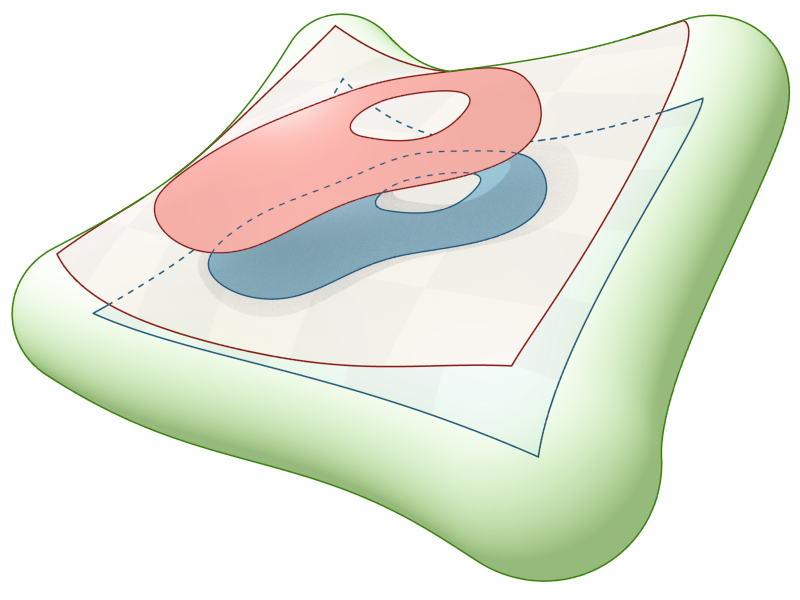
\includegraphics[width=80mm]{EdS_propre_carreau_restreint/EdS_propre_carreau_restreint.png}};
		%\drawGrid{20}{20}{blue, thin, dotted}%%%
		\node[colorFace0] at (0.64, 0.31) {$\carreau$};
		\node[colorFace1] at (0.57, 0.455) {$\EdSpropreplus{\carreau}{\rho}$};
		\node[colorFace0!50!black] at (0.35, 0.55) {$\brepface$};
		\node[colorFace1, anchor=south, inner sep=0] at (0.355, 0.695) {$\EdSpropreplus{\brepface}{\rho}$};
		\node[colorEdS, anchor=west] at (0.81, 0.1) {$\EdS{\carreau}{\rho}$};
		\coordinate (destMap0) at (0.55, 0.3);
		\coordinate (destMap1) at (0.4, 0.93);%(0.375, 0.9);
	\end{scope}
	%
	\begin{scope}[
		x=0.3\imageheight,
		y=0.3\imageheight,
		shift={(-0.5\imageheight,0.5\imageheight)}
	]
		{\transparent{0.035}%
			\drawUVchecker{6}{black}
		}%
		\path[draw=colorBordDomaineUV, fill=colorInterieurDomaineUV, line width=0.6pt]
(0.5265310634108271, 0.438547589973437) .. controls (0.3310295488391929, 0.6935604776607408) and (-0.021382588776948222, 0.7376543228644009) .. (-0.10761414246666436, 0.6458722526584881)
.. controls (-0.21738265636518123, 0.5288877287485011) and (-0.17017248387614453, 0.367245125596702) .. (-0.2879469981322148, 0.19968851382281255)
.. controls (-0.40569858776829065, 0.03213190204887557) and (-0.6468263047931714, -0.04383071753181846) .. (-0.693539828033049, -0.2425873818597733)
.. controls (-0.7509242728775373, -0.48485275979627296) and (-0.41538197233103924, -0.7039845421685414) .. (-0.15341941399581885, -0.6891054816069568)
.. controls (0.1085262173182571, -0.6742682161592514) and (0.16478678736946484, -0.4840377550744662) .. (0.3373277172510478, -0.34364796735972497)
.. controls (0.5098686471326309, -0.20327907720189958) and (0.9385113528049314, -0.09879129235910938) .. (0.5265310634108271, 0.438547589973437)
-- cycle
(0.42885638368115414, 0.1734202847133243) .. controls (0.4481705327582044, -0.06518802075369291) and (0.280929641274987, -0.06594033280456221) .. (0.16421795586878063, -0.05212704764834414)
.. controls (0.047447004991011434, -0.03833466004908937) and (0.03296990893768833, 0.11674611021456661) .. (0.08180520084194194, 0.20877895110413416)
.. controls (0.13056009984453748, 0.3008326895506175) and (0.40950330245547123, 0.4120494877373048) .. (0.42885638368115414, 0.1734202847133243)
-- cycle
;
		\node[colorBordDomaineUV] at (-0.2, -0.25) {$\uvdomain$};
		\draw[axe] (-1,-1) -- ++ (2.05,0) node [below right, axeuvlabel] {$u$};
		\draw[axe] (-1,-1) -- ++ (0,2.05) node [above left, axeuvlabel] {$v$};
		%
		\node[inner sep=0.3] (uvcenter) at (0,0) {};
		\draw[map, colorFace0] (1.05, -0.45) to [bend right=20] node[below] {$\bs$} (destMap0);
		\draw[map, colorFace1] (1.05, 0.45) to [bend left=20] node[above] {$\eos$} (destMap1);
	\end{scope}
\end{tikzpicture}
	\caption{EdS propre d'un carreau paramétrique restreint.}
	\label{fig:EdS_propre_carreau_restreint}
\end{figure}



\subsection{Paramétrisation de la pseudo-EdS d'une arête \brep\ convexe}% arc paramétrique}
%\begin{enumerate}
%	\item détermination de la convexité de l'arête (signe de $\dotprod{\left(\crossprod{\unv_L}{\unv_R}\right)}{\bt}$, \cf \autoref{section:def_convexite_courbe_singuliere})
%	\item rappeler système définissant une EdS propre à 1 paramètre
%	\item notion de cercle caractéristique
%	\item paramétrisation générique $\eos(u,v) = \bo(u) + r(u)\br(u,v)$ de l'EdS propre
%	\item restriction à la portion entre les EdS propres des faces incidentes, paramétrisée sur le domaine $\uvdomain = \left[ \lo{u}, \hi{u} \right] \times \left[ \lo{v}, \hi{v} \right]$
%\end{enumerate}

\subsubsection{Paramétrisation de l'EdS propre d'un arc paramétrique}
\label{section:parametrisation_EdS_propre_courbe}
%\begin{figure}
%	\centering
%	\setlength{\imagewidth}{120mm}%
%	\setlength{\imageheight}{0.6857\imagewidth}%
%	\definecolor{coloreos}{HTML}{64CF36}
%	\definecolor{colorshpere}{HTML}{CD6E33}
%	\begin{tikzpicture}[x=\imagewidth, y=\imageheight]
%		\node[inner sep=0, anchor=south west] {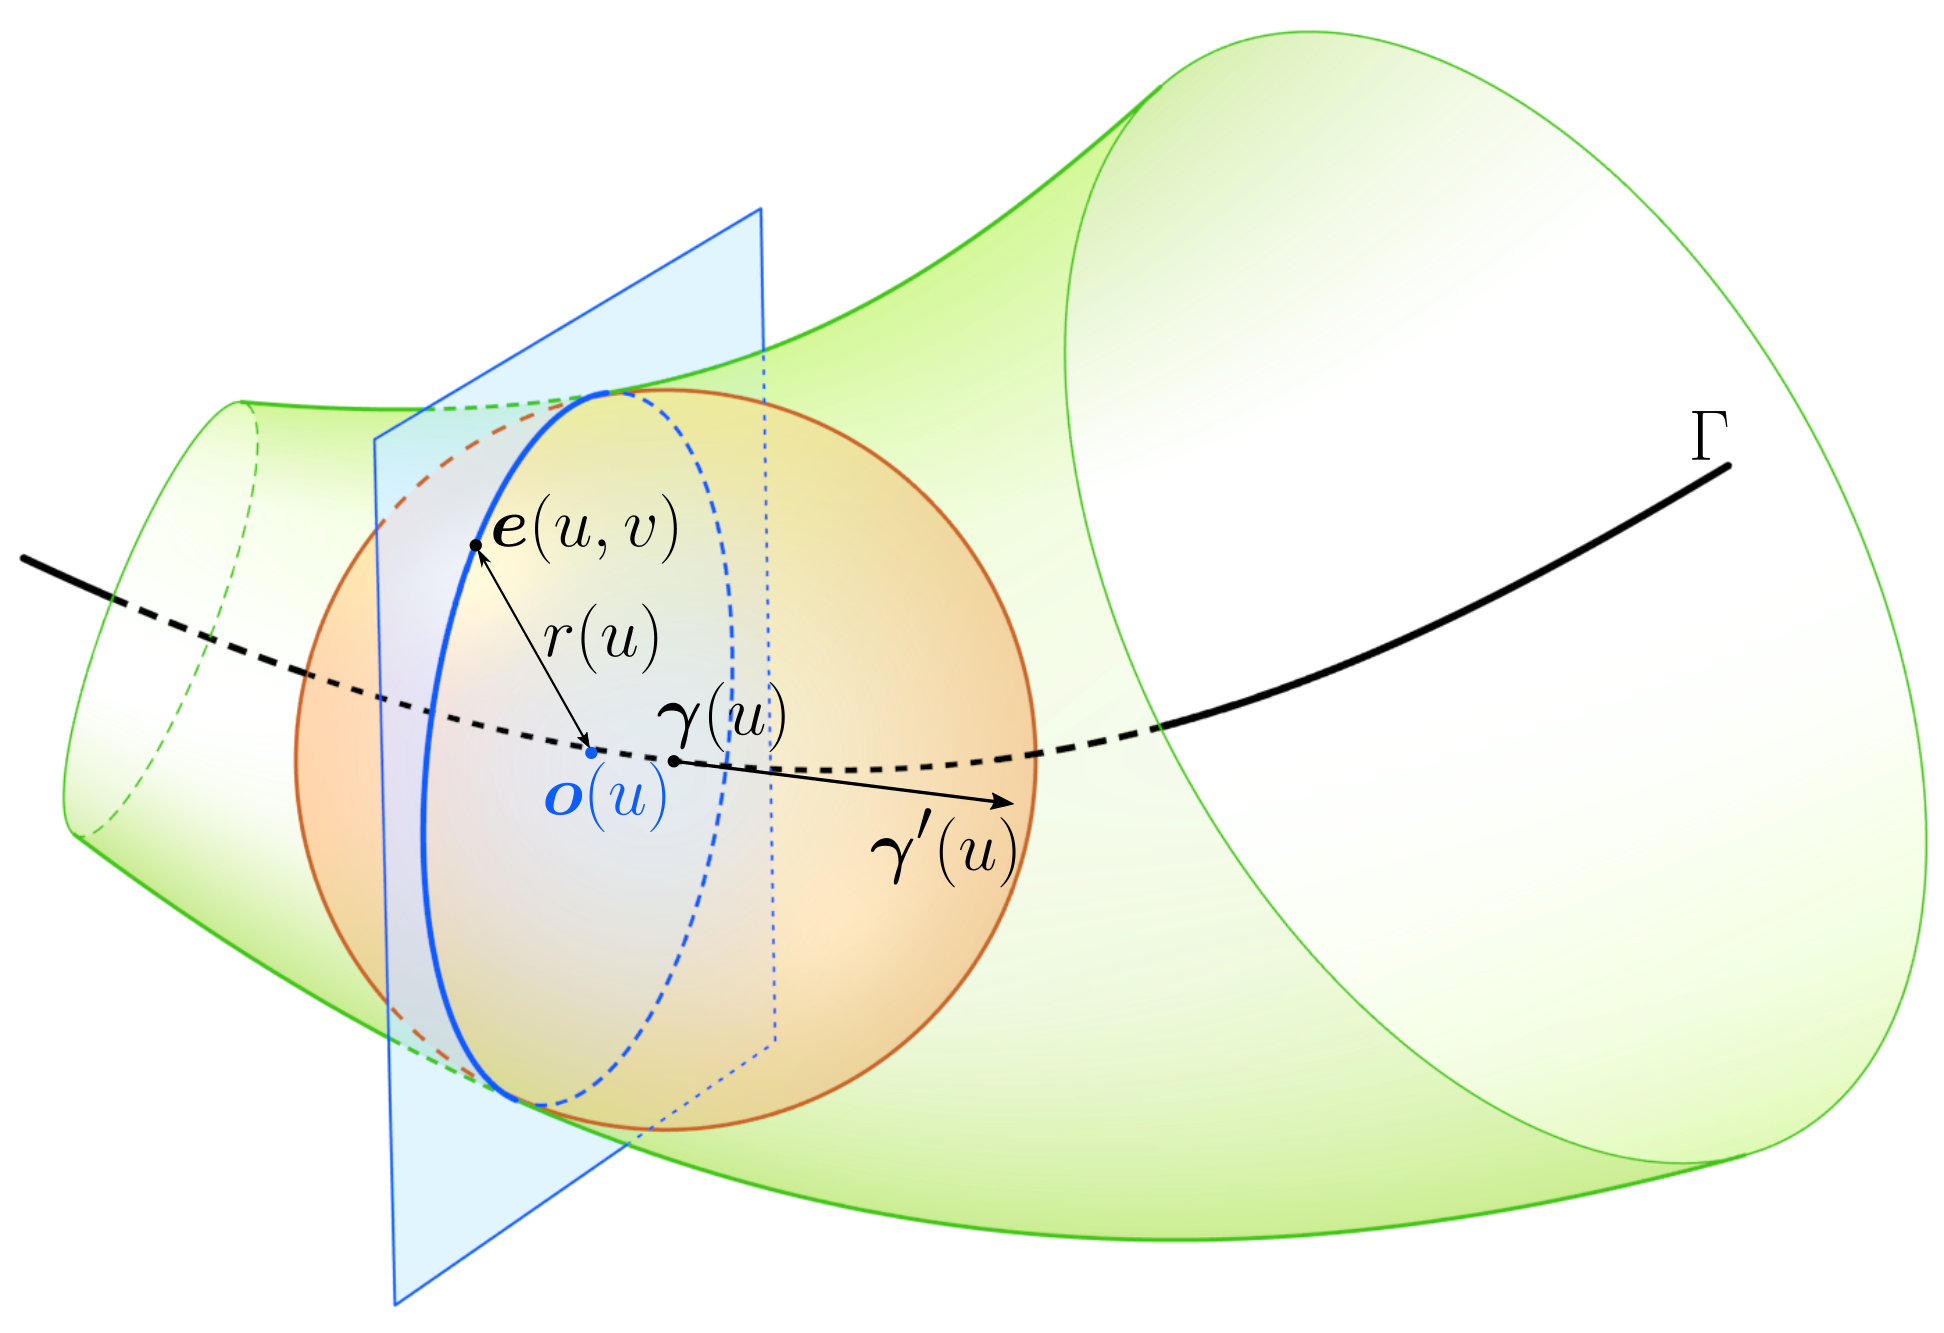
\includegraphics[width=\imagewidth]{figures/images/EdS_propre_courbe.png}};
%		\node[coloreos] at (0.55,0.95) {$\EdSpropre{\Gamma}{\rho}$};
%		\node[anchor=south west, colorshpere] at (0.46,0.62) {$\sphere[u]$};
%	\end{tikzpicture}
%	\caption{Paramétrisation de l'EdS propre d'un arc paramétrique.}
%	%\label{fig:parametrisation_EdS_propre_courbe}
%\end{figure}

\begin{figure}
	\centering%
	\setlength{\imagewidth}{140mm}%
	\setlength{\imageheight}{0.75\imagewidth}%
	\definecolor{colorEdS}{HTML}{64CF36}%
	\colorlet{colorEdSPoint}{black}%colorEdS!75!black}
	\definecolor{colorSphere}{HTML}{CD6E33}%
	\definecolor{colorCercle}{rgb}{0.049, 0.363, 1}%
	\DTLsetseparator{,}%
	\DTLloaddb[noheader,keys={x,y}]{dbspinepttng}{figures/data/EdS_propre_courbe/spine_point_tangent.dat}%
	\DTLloaddb[noheader,keys={x,y}]{dbcirclectrpt}{figures/data/EdS_propre_courbe/circle_center_point.dat}%
	\DTLloaddb[noheader,keys={x,y}]{dbenvelope}{figures/data/EdS_propre_courbe/envelope_data.dat}%
	\begin{tikzpicture}[
		x = \imagewidth,
		y = \imageheight,
		point/.style = {circle, scale=0.27, fill=black},
		vector/.style = {-latex', thick},
		label/.style = {inner sep=2pt},
		txt/.style = {font=\small},
	]
		\begin{scope}
			\clip (0.05,0.13) rectangle (0.95,0.97);	
			%
			\node[anchor=south west, inner sep=0] at (0,0) {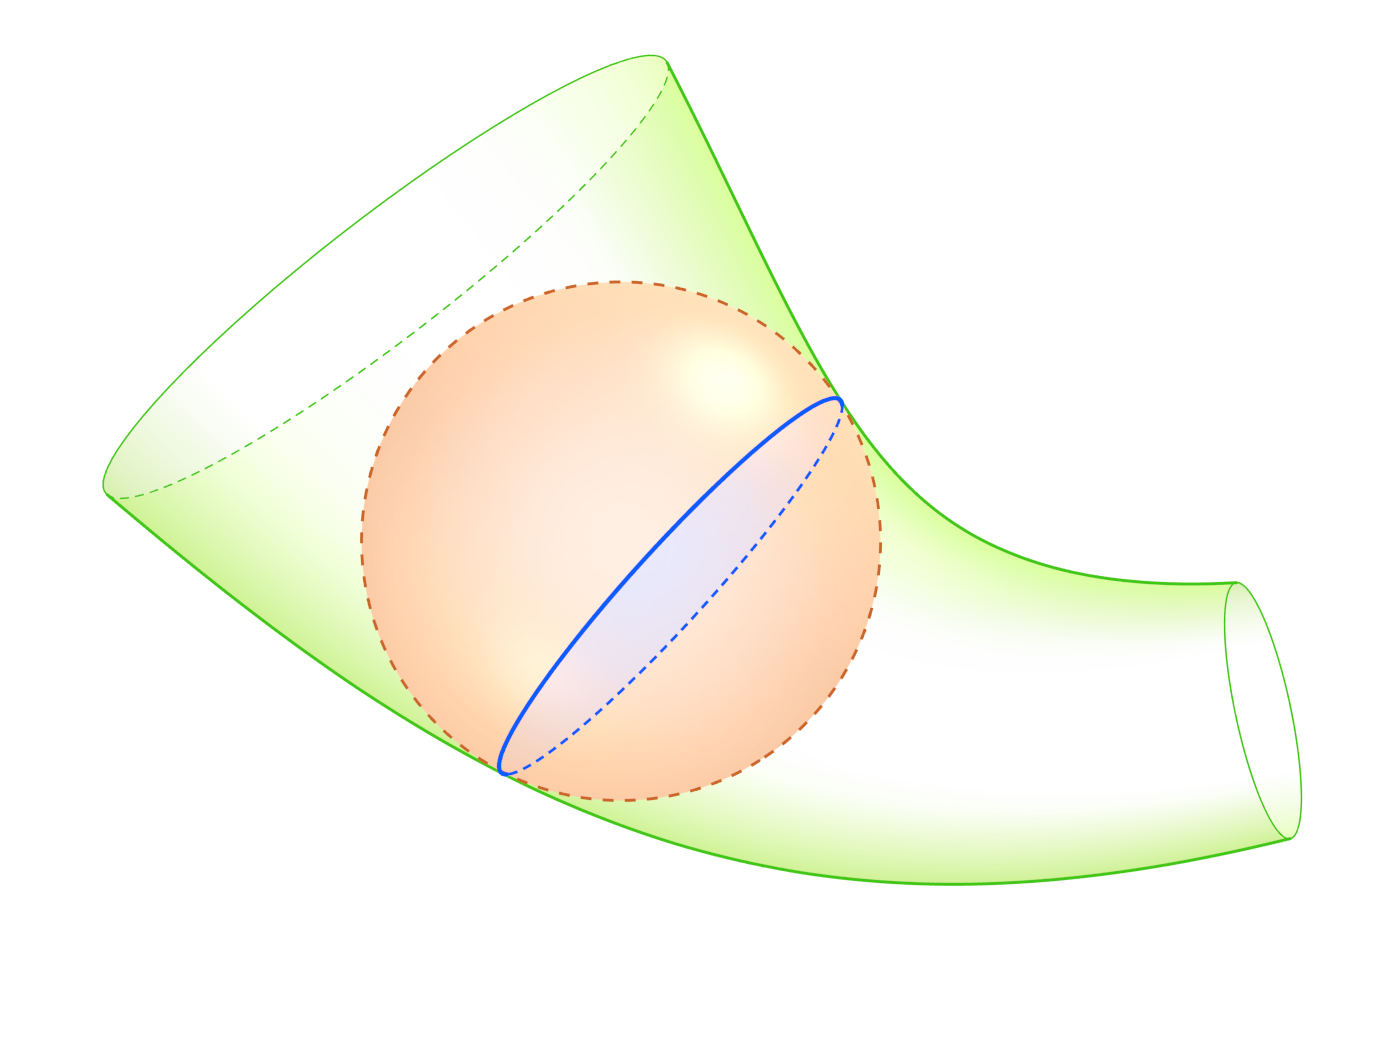
\includegraphics[width=\imagewidth]{figures/images/EdS_propre_courbe/Image0001.png}};
			%
			%\drawGrid{10}{10}{red, thin, dotted}
			%
			\draw[thick, line cap=round] plot file {figures/data/EdS_propre_courbe/spine_xy.dat} node [above right] {$\Gamma$};
			%
			\DTLassign{dbspinepttng}{1}{\gx=x, \gy=y}%
			\coordinate (g) at (\gx, \gy);
			\DTLassign{dbspinepttng}{2}{\dgx=x, \dgy=y}%
			\coordinate (dg) at (\dgx, \dgy);
			\draw[vector] (g) -- (dg) node[txt, below] {$\bg'(u)$};
			\node[txt, left] at (g) {$\bg(u)$};
			\node[point] at (g) {};
			%
			\DTLassign{dbcirclectrpt}{1}{\occx=x, \occy=y}%
			\coordinate (occ) at (\occx, \occy);
			\node[txt, below left, inner sep=0, colorCercle, shift={(1pt,-1pt)}] at (occ) {$\vit{o}(u)$};
			%
			\DTLassign{dbenvelope}{1}{\edsx=x, \edsy=y}%
			\node[colorEdS, above] at (\edsx, \edsy) {$\EdSpropre{\Gamma}{\rho}$};
			%
			\DTLassign{dbenvelope}{2}{\ex=x, \ey=y}%
			\coordinate (e) at (\ex, \ey);
			\node[txt, left, colorEdSPoint] at (e) {$\eos(u,v)$};
			%\draw [dotted, thick, <-, ->] (occ) -- node[txt, right] {$r(u)$} (e);
			\draw [dotted, thick] (occ) -- (e);
			\node[point, fill=colorCercle] at (occ) {};
			%
			\DTLassign{dbenvelope}{3}{\rx=x, \ry=y}%
			\coordinate (r) at (\rx, \ry);
			\draw[vector] (e) -- (r) node[txt, right] {$\vrm{r}(u,v)$};
			\node[point, colorEdSPoint] at (e) {};
			\node[colorSphere] at (0.31,0.55) {$\sphere[u]$};
			%
			\DTLassign{dbenvelope}{4}{\cx=x, \cy=y}%
			\coordinate (c) at (\cx, \cy);
			\node[txt, left, colorCercle] at (c) {$\circlenotation(u)$};
		\end{scope}
		%
		%\draw[red, dotted, thin] (current bounding box.south west) rectangle (current bounding box.north east);
	\end{tikzpicture}
	\DTLgdeletedb{dbspinepttng}%
	\DTLgdeletedb{dbcirclectrpt}%
	\DTLgdeletedb{dbenvelope}%
	\caption{Paramétrisation de l'EdS propre d'un arc paramétrique.}%
	\label{fig:parametrisation_EdS_propre_courbe}%
\end{figure}

%%Soit $\bg : \wdomain \to \reals^3$ une paramétrisation du support géométrique $\Gamma$ de l'arête $\brepedge$. 
%%L'EdS propre de $\Gamma$ est le lieu des points $\bx \in \reals^3$ qui vérifient
%L'enveloppe $\Phi$ d'une famille de sphères à un paramètre centrées sur une courbe directrice $\Gamma$ est appelée \textit{surface canal} \cite{monge1850}. 
%Si la $\Gamma$ dispose d'une paramétrisation $\bg : \wdomain \to \reals^3$ alors cette surface est le lieu des points $\bx \in \reals^3$ qui vérifient
%\begin{equation}
%  \left\{
%    \begin{matrix}
%        \normtwo{\bx - \bg(u)}^2 - \rho(u)^2 &= 0 ,\\ 
%        \dotprod{\left(  \bx - \bg(u) \right)}{\bg'(u)} + \rho(u)\rho_u(u) &= 0.
%    \end{matrix}
%  \right.
%  \label{eq:sys_canal_surface}
%\end{equation}
Soit $\bg : \left[ \lo{u}, \hi{u} \right] \to \reals^3$ une paramétrisation du support géométrique $\Gamma$ de l'arête $\brepedge$. 
Si l'on considère $\rho$ comme une fonction du paramètre $u$ alors $\EdSpropre{\Gamma}{\rho}$ est le lieu des points $\bx \in \reals^3$ qui vérifient
%\begin{equation}
%  \left\{
%    \begin{matrix}
%        \normtwo{\bx - \bg(u)}^2 - \rho(u)^2 &= 0 ,\\ 
%        \dotprod{\left(  \bx - \bg(u) \right)}{\bg'(u)} + \rho(u)\rho_u(u) &= 0.
%    \end{matrix}
%  \right.
%  \label{eq:sys_canal_surface}
%\end{equation}
\begin{subequations}
	\label{eq:sys_canal_surface}
	\begin{empheq}[left={\empheqlbrace\,}]{align}
		\normtwo{\bx - \bg(u)}^2 - \rho(u)^2 &= 0 ,\\ 
		\dotprod{\left(  \bx - \bg(u) \right)}{\bg'(u)} + \rho(u)\rho_u(u) &= 0.
	\end{empheq}
\end{subequations}	
A condition que $\rho_u^2 \leq \normtwo{\bg'}^2$, le système \eqref{eq:sys_canal_surface} définit une famille de \textit{cercles caractéristiques}, dont chacun est le lieu des points de tangence entre $\EdSpropre{\Gamma}{\rho}$ et une sphère de la famille $\sphere[\Gamma][\rho]$ (voir \autoref{fig:parametrisation_EdS_propre_courbe}).
\par
D'après \eqref{eq:sys_canal_surface}, le cercle caractéristique $\circlenotation(u)$ au point $\bg(u)$ est l'intersection de la sphère $\sphere[u] = \sphere[\bg(u)][\rho(\bg(u))]$ et d'un plan orthogonal à la direction tangente à $\Gamma$ en ce point (donnée par le vecteur $\bg'(u)$). 
Ce cercle est centré en
\begin{equation}
    \bo(u) = \bg(u) - \frac{\rho(u)\rho_u(u)}{\normtwo{\bg'(u)}^2} \bg'(u),
    \label{eq:cercle_caracteristique_centre}
\end{equation}
et a pour rayon
\begin{equation}
    r(u) = \rho(u) \sqrt{1 - \frac{\rho_u(u)^2}{\normtwo{\bg'(u)}^2}}.
    \label{eq:cercle_caracteristique_rayon}
\end{equation}
\par
Voir $\EdSpropre{\Gamma}{\rho}$ comme une famille cercles caractéristiques permet d'en donner la paramétrisation suivante
\begin{equation}
    \eos(u,v) = \bo(u) + r(u)\br(u,v),
    \label{eq:parametrisation_EdS_propre_courbe}
\end{equation}
où $\br$ vérifie
\begin{equation}
	\left\{
		\begin{matrix}
			\normtwo{\br} = 1,\\ 
			\dotprod{\br}{\bg'} = 0.
		\end{matrix}
	\right.
	\label{eq:parametrisation_EdS_propre_courbe_condition_r}
\end{equation}
De cette façon, les courbes iso-$u$ de $\eos$ sont les cercles caractéristiques.


\subsubsection{Paramétrisation de la pseudo-EdS}
\label{section:parametrisation_pseudo_EdS_arete}

%\begin{figure}
%    \centering
%    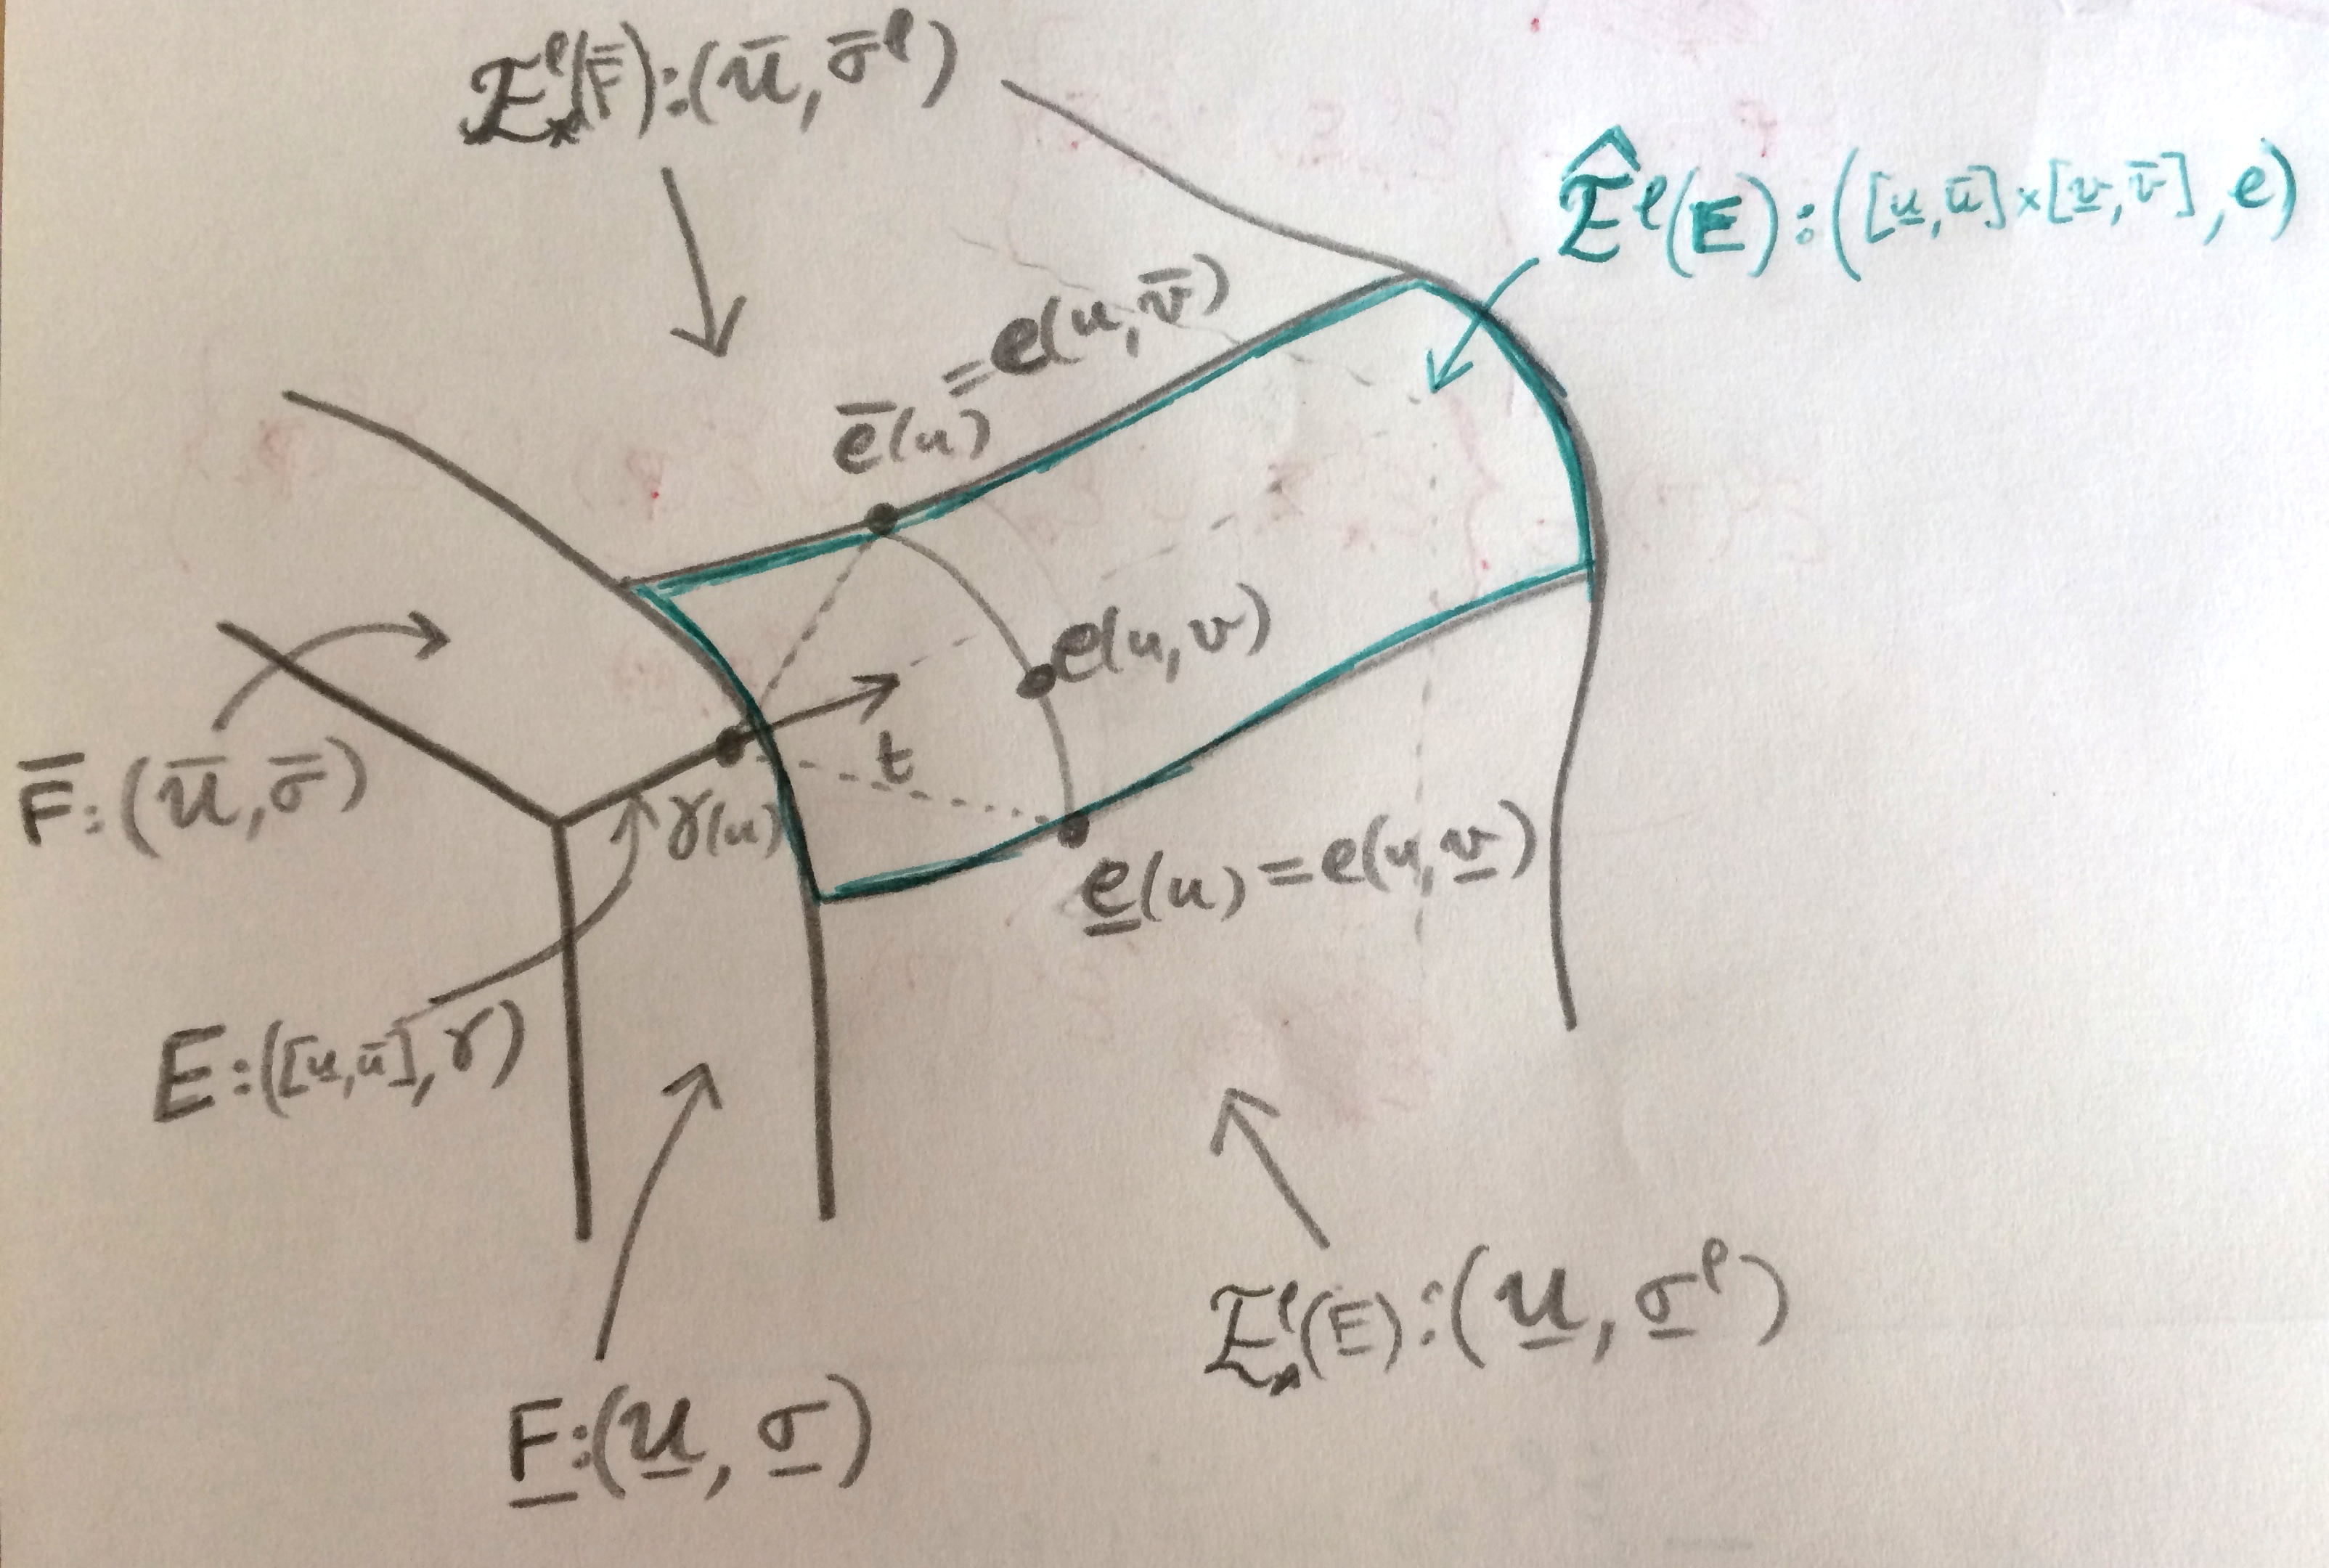
\includegraphics[width=10cm]{pseudo-EdS_arete.JPG}
%    \caption{Paramétrisation de $\pseudoEdS{\brepedge}{\rho}$}
%    \label{fig:pseudo-EdS_arete}
%\end{figure}
\begin{figure}
    \centering
    \setlength{\imagewidth}{120mm}%
	\setlength{\imageheight}{0.75\imagewidth}%
	%
	\colorlet{colorRight}{mycolor_2!70!black}
	\colorlet{colorLeft}{mycolor_3!85!black}
	\colorlet{colorPseudoEdS}{mycolor_4!80!black}
	\colorlet{colorAngle}{yellow!20!white}%mycolor_5!12!white}
	%
	\DTLsetseparator{,}%
	\DTLloaddb[noheader,keys={x,y}]{dbisoupoints}{figures/data/pseudo_EdS_arete/iso-u_points.dat}%
    \begin{tikzpicture}[
    	x=\imagewidth,
		y=\imageheight,
		curve/.style = {thick, line cap = round},
		point/.style = {circle, scale=0.27, fill=black},
		vector/.style = {-latex', thick},
		label/.style = {inner sep=2pt},
		txt/.style = {font=\small},
		insert node/.style args={#1 at #2}{
    		postaction=decorate,
    		decoration={
      			markings,
      			mark= at position #2 with {#1}
      		}
		}
    ]
    	%
    	\node[anchor=south west, inner sep=0] {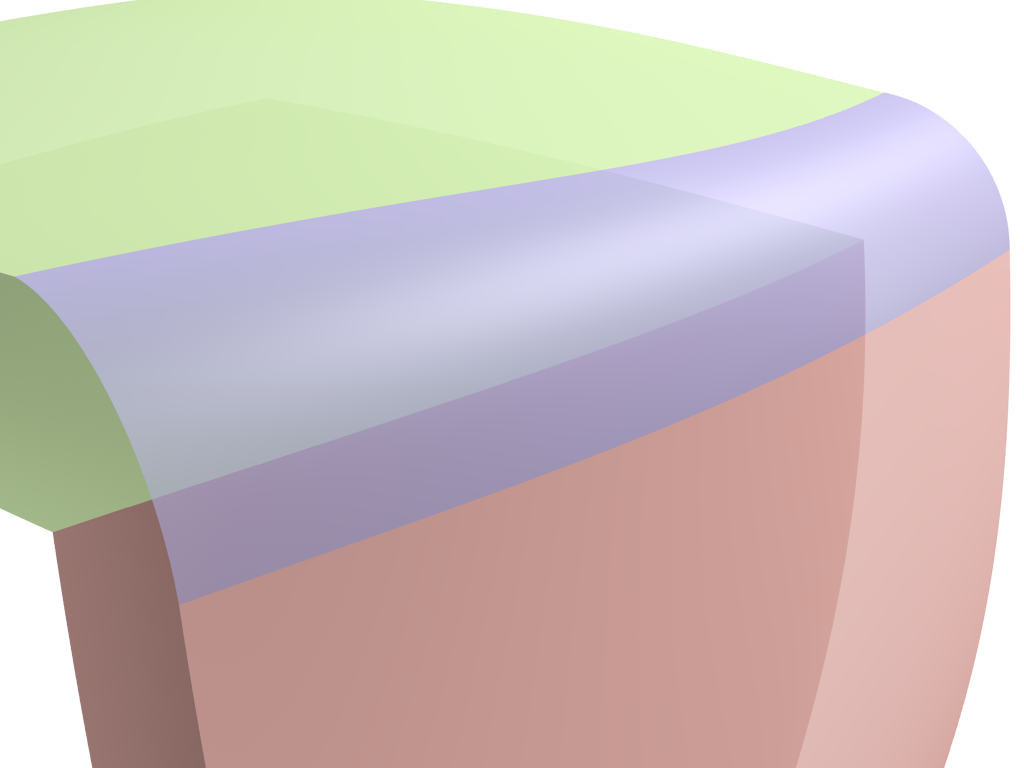
\includegraphics[width=\imagewidth]{pseudo_EdS_arete/pseudo_EdS_arete0001.png}};
    	%
    	{\transparent{0.6}%
    		\draw[curve, dash pattern=on 3pt off 4pt] plot file {figures/data/pseudo_EdS_arete/edge_hidden.dat};
    	}%
    	\draw[
    		curve,
    		insert node={\node[txt, above] {$\brepedge$};} at 0.2,
    		shorten <= 0.4pt
    	] plot file {figures/data/pseudo_EdS_arete/edge_visible.dat};
    	%
    	% iso-v curves (boundary curves)
    	\draw[curve, colorRight] plot file {figures/data/pseudo_EdS_arete/iso-v_curve_0.dat};
    	\draw[curve, colorLeft!90!black] plot file {figures/data/pseudo_EdS_arete/iso-v_curve_1.dat};
    	%
    	% iso-u curve
    	\draw[curve, colorPseudoEdS] plot file {figures/data/pseudo_EdS_arete/iso-u_curve.dat};
    	%
		% points on iso-u curve
		\DTLassign{dbisoupoints}{1}{\ex=x, \ey=y}%
		\coordinate (e) at (\ex, \ey);
		\node[txt, right, colorPseudoEdS!70!black] at (e) {$\eos(u,v)$};
		%
		\DTLassign{dbisoupoints}{2}{\eRx=x, \eRy=y}%
		\coordinate (eR) at (\eRx, \eRy);
		\node[txt, below, colorRight!70!black] at (eR) {$\Right{\eos}(u)$};
		%
		\DTLassign{dbisoupoints}{3}{\eLx=x, \eLy=y}%
		\coordinate (eL) at (\eLx, \eLy);
		\node[txt, above left, inner sep=1pt, colorLeft!70!black] at (eL) {$\Left{\eos}(u)$};
		%
%		\DTLassign{dbisoupoints}{4}{\enx=x, \eny=y}%
%		\coordinate (en) at (\enx, \eny);
%		\draw[vector] (e) -- (en) node[txt, left, inner sep=1pt] {$\unv_{\envelope}(u,v)$};
		%
		\DTLassign{dbisoupoints}{5}{\occx=x, \occy=y}%
		\coordinate (occ) at (\occx, \occy);
		\node[txt, above left, inner sep=0, colorPseudoEdS!90!black] at (occ) {$\bo(u)$};
		\draw[dotted, thick, colorPseudoEdS] (occ) -- (e);
		\draw[dotted, thick, colorRight] (occ) -- (eR);
		\draw[dotted, thick, colorLeft!80!black] (occ) -- (eL);
		%
		\DTLassign{dbisoupoints}{6}{\gx=x, \gy=y}%
		\coordinate (g) at (\gx, \gy);
		\node[txt, below] at (g) {$\bg(u)$};
		%
		\DTLassign{dbisoupoints}{7}{\tx=x, \ty=y}%
		\coordinate (t) at (\tx, \ty);
		\draw[vector] (g) -- (t) node[txt, below right, inner sep=0, shift={(-2pt,-1pt)}] {$\bt(u)$};
		%
		\DTLassign{dbisoupoints}{8}{\rx=x, \ry=y}%
		\coordinate (r) at (\rx, \ry);
		\draw[vector, colorPseudoEdS] (e) -- (r) node[txt, right, inner sep=1pt] {$\br(u,v)$};
		%
		\DTLassign{dbisoupoints}{9}{\rRx=x, \rRy=y}%
		\coordinate (rR) at (\rRx, \rRy);
		\draw[vector, colorRight] (eR) -- (rR) node[txt, right, inner sep=1pt] {$\Right{\br}(u)$};
		%
		\DTLassign{dbisoupoints}{10}{\rLx=x, \rLy=y}%
		\coordinate (rL) at (\rLx, \rLy);
		\draw[vector, colorLeft] (eL) -- (rL) node[txt, right] {$\Left{\br}(u)$};
		%
		\node[txt, colorRight] at (0.92,0.38) {$\EdSpropreplus{\Right{\brepface}}{\rho}$};
		\node[txt, colorLeft] at (0.6,0.9) {$\EdSpropreplus{\Left{\brepface}}{\rho}$};
		\node[txt, colorPseudoEdS] at (0.9,0.75) {$\pseudoEdS{\brepedge}{\rho}$};
		%
		\node[txt, colorRight!50!black] at (0.13,0.15) {$\Right{\brepface}$};
		\node[txt, colorLeft!50!black] at (0.055,0.47) {$\Left{\brepface}$};
		%
		%
		\node[point, colorPseudoEdS!70!black] at (e) {};
		\node[point, colorRight!70!black] at (eR) {};
		\node[point, colorLeft!70!black] at (eL) {};
		\node[point, colorPseudoEdS!90!black] at (occ) {};
		\node[point] at (g) {};
		%
		% angle anotation
		\draw[
			colorAngle,
			insert node={\node[txt, right] {$\theta(u)$};} at 0.68,
			curve, 
			-{Triangle[length=4pt, width=4pt]}, 
			line width=0.6pt, 
		] plot file {figures/data/pseudo_EdS_arete/angle_anotation.dat};
		%
		%
		%\drawGrid{10}{10}{thin, dotted}
	\end{tikzpicture}
    \DTLgdeletedb{dbisoupoints}%
    \caption{Paramétrisation de la pseudo-EdS d'une arête \brep\ convexe.}%$\pseudoEdS{\brepedge}{\rho}$}
    \label{fig:pseudo-EdS_arete}
\end{figure}

\begin{enumerate}
	\item $\brepedge$ une arête convexe du modèle \brep\ de $\Sigma$, $\bg : \left[ \lo{u}, \hi{u} \right] \to \reals^3$ une paramétrisation de son support géométrique
	\item $\Right{\brepface}$ (resp. $\Left{\brepface}$) la face à gauche\footnote{relativement à l'orientation donnée par $\bg$, vu de l'extérieur de $\Omega$.} (resp. à droite) de $\brepedge$
	\item but : construire une paramétrisation $\eos$ de la pseudo-EdS de $\brepedge$, \ie la région $\pseudoEdS{\brepedge}{\rho}$ de $\EdS{\brepedge}{\rho}$ qui est tangente à la fois à $\EdS{\Right{\brepface}}{\rho}$ et $\EdS{\Left{\brepface}}{\rho}$ (voir \autoref{fig:pseudo-EdS_arete})
	\item on note $\Right{\bs}$ (resp. $\Left{\bs}$) une paramétrisation du carreau supportant $\Right{\brepface}$ (resp. $\Left{\brepface}$) et $\Right{\bp}$ (resp. $\Left{\bp}$) une paramétrisation de la trace de $\brepedge$ dans l'espace paramétrique de $\Right{\brepface}$ (resp. de $\Left{\brepface}$) telle que
	\begin{equation}
	    \bg = \Right{\bs} \circ \Right{\bp} = \Left{\bs} \circ \Left{\bp}.
	\end{equation}
	\item on note $\Right{\EdB{\bs}{\rho}}$ (resp. $\Left{\EdB{\bs}{\rho}}$) la paramétrisation de $\EdSpropreplus{\Right{\brepface}}{\rho}$ (resp. de $\EdSpropreplus{\Left{\brepface}}{\rho}$) obtenue comme décrit dans la \autoref{section:parametrisation_eds_propre_face}. 
	\item enfin, on note
	\begin{equation}
	    \Right{\eos} = \Right{\EdB{\bs}{\rho}} \circ \Right{\bp} \quad\text{et}\quad \Left{\eos} = \Left{\EdB{\bs}{\rho}} \circ \Left{\bp}.
	    \label{eq:pseudoEdSarete_courbes_limites}
	\end{equation}
	
	\item On choisit une paramétrisation de la forme \eqref{eq:parametrisation_EdS_propre_courbe}, \ie les courbes iso-$u$ sont des arcs de cercles caractéristiques dont les extrémités $\Right{\eos}$ et $\Left{\eos}$ sont respectivement atteintes en $v = \lo{v}$ et $v = \hi{v}$. 
Le domaine paramétrique du carreau décrivant $\pseudoEdS{\brepedge}{\rho}$ est donc le rectangle $\mathcal{U} = \left[ \lo{u}, \hi{u} \right] \times \left[ \lo{v}, \hi{v} \right]$.

	%\item on suppose que l'on peut évaluer $\bg(u)$, $\Right{\eos}(u)$ et $\Left{\eos}(u)$ pour tout $u \in \left[ \lo{u}, \hi{u} \right]$
	
	\item on propose alors une méthode pour construire une telle paramétrisation qui n'exploite pas directement la donnée de $\rho$ et $\rho_u$ mais plutôt celle de $\Right{\eos}(u)$ et $\Left{\eos}(u)$ (ce choix, qui sera motivé lors de la mise en \oe uvre numérique, garantit que $\eos(u,\lo{v}) = \Right{\eos}(u)$ et $\eos(u,\hi{v}) = \Left{\eos}(u)$)

	\item on note $\bt = \unitized{\bg'}$ et $\mu = -\frac{\rho \rho_u}{\normtwo{\bg}}$, on a alors $\bo = \bg + \mu \bt$
	
	\item or $\mu = \dotprod{\left( \Right{\eos} - \bg \right)}{\bt} = \dotprod{\left( \Left{\eos} - \bg \right)}{\bt}$ %(pour l'implémentation, on choisit $\mu = \frac{1}{2} \dotprod{\left( \Right{\eos} + \Left{\eos} - 2 \bg\right)}{\bt}$)
		
	\item on a $r = \normtwo{\Right{\eos} - \bo} = \normtwo{\Left{\eos} - \bo}$ (rayon du cercle caractéristique) %(pour l'implémentation, on choisit $r(u,v) = \left( 1 - \frac{v - \lo{v}}{\hi{v} - \lo{v}} \right) \normtwo{\Right{\eos} - \bo} + \frac{v - \lo{v}}{\hi{v} - \lo{v}} \normtwo{\Left{\eos} - \bo}$)
	
	\item on note $\Right{\br} = \unitized{\Right{\eos} - \bo}$ et $\Left{\br} = \unitized{\Left{\eos} - \bo}$
	
	\item on définit $\Right{\br}^{\perp} = \crossprod{\Right{\br}}{\bt}$ (de telle sorte que $\left( \Right{\br}, \Left{\br}^{\perp}, -\bt \right)$ forme un trièdre orthonormé direct)
	
	\item on note $\theta \in \left[0, 2\pi\right[$ l'angle entre les vecteurs $\Right{\br}$ et $\Left{\br}$ mesuré dans le sens direct autour de $-\bt$, \ie
	\begin{equation}
	    \theta = 
	    \begin{cases}
	       \vartheta + 2\pi & \text{ si } \vartheta < 0, \\ 
	       \vartheta        & \text{ si } \vartheta \geq 0,
	    \end{cases}
	\end{equation}
	où
	\begin{equation}
		\vartheta = \arctan \left(
			\frac{
        		\dotprod{\Left{\br}}{\Right{\br}^{\perp}}    	
			}{
				\dotprod{\Left{\br}}{\Right{\br}}
			}
		\right).
	\end{equation}
	
	\item Enfin, on choisit une paramétrisation naturelle pour l'arc de cercle caractéristique $\eos(u, \left[\lo{v},\hi{v}\right])$, \ie
%	\begin{equation}
%	    \br(u,v) = 
%	        \cos\left( \lambda(v) \theta(u) \right) \Right{\br}(u) +
%	        \sin\left( \lambda(v) \theta(u) \right) \Right{\br}^{\perp}(u),
%	\end{equation}
%	avec 
%	\begin{equation}
%	    \lambda(v) = \frac{v - \lo{v}}{\hi{v} - \lo{v}} \in \left[0, 1\right].
%	\end{equation}
	\begin{equation}
	    \br(u,v) = 
	        \cos\left( \frac{v - \lo{v}}{\hi{v} - \lo{v}} \theta(u) \right) \Right{\br}(u) +
	        \sin\left( \frac{v - \lo{v}}{\hi{v} - \lo{v}} \theta(u) \right) \Right{\br}^{\perp}(u).
	\end{equation}	
	De cette façon, $\br$ vérifie bien les conditions \eqref{eq:parametrisation_EdS_propre_courbe_condition_r} et on a bien $\br(u,\lo{v}) = \Right{\br}(u)$ et $\br(u,\hi{v}) = \Left{\br}(u)$ (donc $\eos(u,\lo{v}) = \Right{\eos}(u)$ et $\eos(u,\hi{v}) = \Left{\eos}(u)$).
	
	\item \textit{Remarque :} si une extrémité de $\brepedge$ est un point régulier de $\Sigma$ alors l'arc de cercle caractéristique en cette extrémité est réduit à un seul point et la paramétrisation $\eos$ y est singulière\\
	$\to$ un moyen d'y remédier serait d'utiliser un carreau restreint (\ie les courbes $\Right{\eos}$ et $\Left{\eos}$ ne correspondent plus aux courbes $v = \lo{v}$ et $v = \hi{v}$)
	
\end{enumerate}



\subsection{Paramétrisation de la pseudo-EdS d'un sommet \brep\ convexe}
\def\v{\vit{v}}

%Soit $\brepvertex$ un sommet convexe du modèle \brep\ de $\Sigma$ dont le support géométrique est le point $\v \in \reals^3$. 
%On cherche à construire un ou plusieurs carreaux paramétriques (restreints ou non) décrivant $\pseudoEdS{\v}{\rho}$ \ie la région de la sphère $\sphere[\v][\rho(\v)]$ délimitée par les arcs de cercles caractéristiques aux extrémités des arêtes \brep\ incidentes à $\brepvertex$.\par
%On propose deux approches, en en donnant le principe ainsi que les avantages et les inconvénients.

La pseudo-EdS $\pseudoEdS{\brepvertex}{\rho}$ d'un sommet convexe $\brepvertex$ ayant pour support géométrique le point $\v$ est la région de la sphère $\sphere[\v][\rho(\v)]$ qui est tangente à l'EdS de chacune des arêtes $\family{\brepedge}{i}{1}{m}$ incidentes à $\brepvertex$.
Cette région est le lieu des points $\bx$ vérifiant 
\begin{subequations}
	\label{eq:sys_pseudoEdS_sommet}
	\begin{empheq}[left={\empheqlbrace\,}]{align}
		\normtwo{\bx - \v} &= \rho(\v), \\ 
		\dotprod{\left(  \bx - \lo{\bo}_i \right)}{\lo{\bt}_i} &\leq 0 \quad (i = 1, \ldots, m), 
	\end{empheq}
\end{subequations}

%où $\lo{\bo}_i$ et $\lo{\bt}_i$ désignent respectivement le centre et la normale au plan contenant le cercle caractéristique de l'arête incidente $\brepedge_i$ en son extrémité correspondant à $\brepvertex$ (\cf \autoref{section:parametrisation_pseudo_EdS_arete}).
où $\lo{\bo}_i$ désigne le centre du cercle caractéristique de l'arête incidente $\brepedge_i$ en son extrémité correspondant à $\brepvertex$ et $\lo{\bt}_i$ la normale au plan contenant ce cercle, orientée vers l'intérieur de $\brepedge_i$ (\cf \autoref{section:parametrisation_pseudo_EdS_arete}).
\par
$\pseudoEdS{\brepvertex}{\rho}$ est donc l'intersection de $\sphere{\v}{\rho(\v)}$ et de $m$ demi-espaces délimités par les plans contenant les arcs de cercles caractéristiques des arêtes incidentes.
\par
Si $\gradient{\rho}(\v) = \vit{0}$ alors $\lo{\bo}_i = \v$  pour $i = 1, \ldots, m$ donc ces arcs caractéristiques sont des arcs de grands cercles sur $\sphere[\v][\rho(\v)]$ et donc $\pseudoEdS{\brepvertex}{\rho}$ est un polygone sphérique. 
En revanche, dans le cas général ces plans ne passent pas par $\v$.
\par
On cherche à construire un ou plusieurs carreaux paramétriques (restreints ou non) décrivant $\pseudoEdS{\v}{\rho}$.
Afin de simplifier cette construction, on suppose sans restreindre la généralité que $\v$ est situé à l'origine et que $\rho(\v) = 1$. 
On peut toujours se ramener à ce cas à l'aide d'une transformation adéquate (translation et homothétie) que l'on inversera en fin de construction pour se placer à nouveau dans le cas général.
\par
On suppose également que les arêtes $\family{\brepedge}{i}{1}{m}$ et les faces $\family{\brepface}{i}{1}{m}$ incidentes à $\brepvertex$ sont ordonnées dans le sens direct autour de $\brepvertex$, vu de l'extérieur de $\Omega$ (voir \autoref{fig:cycle_aretes_faces_incidentes}).
\par
On propose deux approches, en en donnant le principe ainsi que les avantages et les inconvénients.

\begin{figure}
	\centering
	\setlength{\imagewidth}{100mm}%
	\setlength{\imageheight}{\imagewidth}%
	\newdimen\radiuscycle
	\radiuscycle=0.08\imagewidth
	%
	\DTLsetseparator{,}%
	\DTLloaddb[noheader,keys={x,y}]{dbvertex}{figures/data/pseudo_EdS_sommet/xy_vertex.dat}%
	\DTLloaddb[noheader,keys={x,y}]{dbfacelabel}{figures/data/pseudo_EdS_sommet/xy_facelabel.dat}%
	\DTLloaddb[noheader,keys={x,y}]{dbedgelabel}{figures/data/pseudo_EdS_sommet/xy_edgelabel.dat}%
	\begin{tikzpicture}[
		x=\imagewidth,
		y=\imageheight
	]
		%
		\node[anchor=south west, inner sep=0] at (0,0) {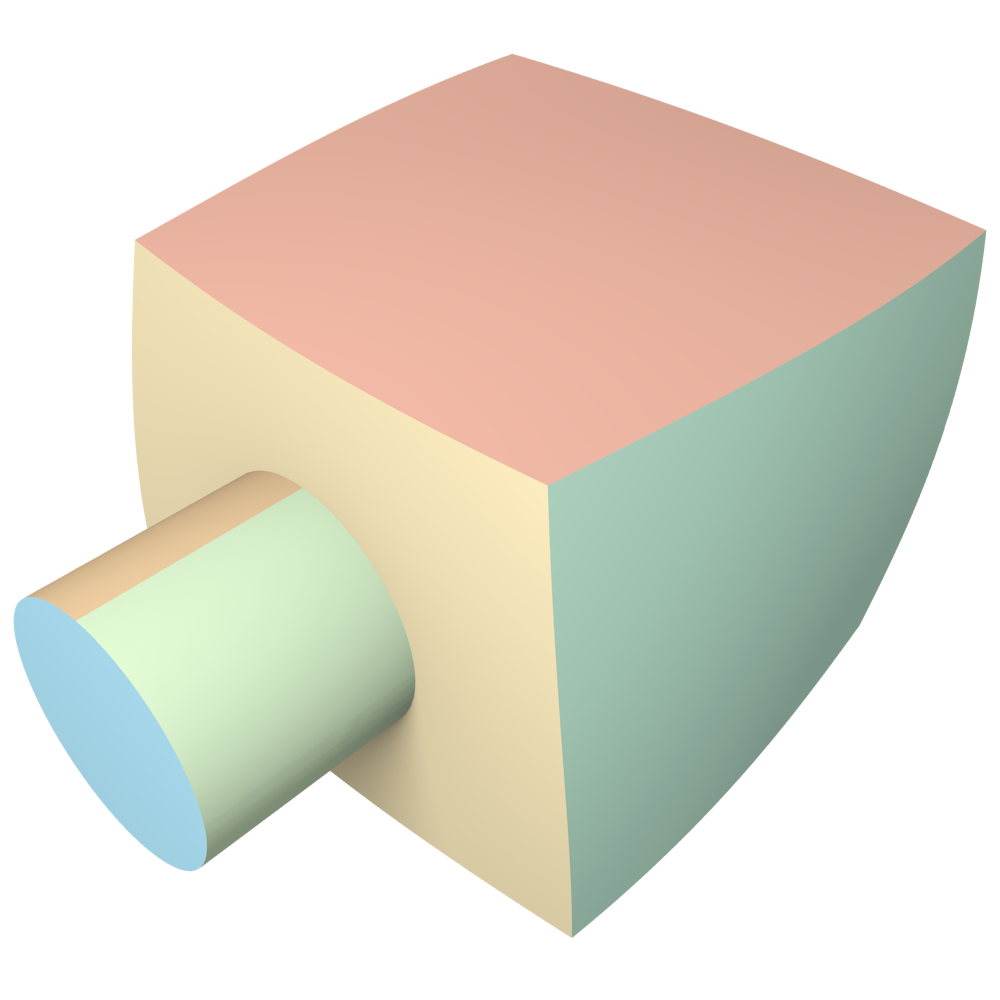
\includegraphics[width=\imagewidth]{pseudo_EdS_sommet/aretes_faces_incidentes}};
		%
		\DTLassign{dbvertex}{1}{\vx=x, \vy=y}%
		\coordinate (v) at (\vx, \vy);
		\fill[black] (v) circle (1.3pt);
		\draw[->] (v) + (-60:\radiuscycle) arc (-60:240:\radiuscycle);
		%
		{\transparent{0.55}%
			\DTLforeach{dbfacelabel}{\flx=x, \fly=y}%
			{%
				\node at (\flx, \fly) {$\brepface_{\arabic{DTLrowi}}$};
			}%
		}
		%
		\DTLforeach{dbedgelabel}{\elx=x, \ely=y}%
		{%
			\node at (\elx, \ely) {$\brepedge_{\arabic{DTLrowi}}$};
			\draw[line width=0.7pt, line cap=round, shorten >= 0.35pt] 
				plot file {figures/data/pseudo_EdS_sommet/xy_edge_\arabic{DTLrowi}.dat};
		}%
		%
		\node[above] at (v) {$\brepvertex$};
	\end{tikzpicture}
	\DTLgdeletedb{dbvertex}%
	\DTLgdeletedb{dbfacelabel}%
	\DTLgdeletedb{dbedgelabel}%
	\caption{Cycle des arêtes et faces incidentes à un sommet du modèle \brep.}
	\label{fig:cycle_aretes_faces_incidentes}
\end{figure}

\subsubsection{Ajustement de plusieurs carreaux non-restreints}%Polygone sphérique découpé en quadrilatères}
\label{section:quadrangulation_polygone_spherique}
Dans un premier temps, on suppose que $\rho$ est uniforme sur $\Sigma$. 

\begin{enumerate}
	%\item hypothèse : $\rho$ est uniforme sur $\Sigma$
	\item[$\Rightarrow$] $\pseudoEdS{\v}{\rho}$ est alors le polygone sphérique formé par les $m$ points $\p_i = \v + \rho \unv_i$, où $\unv_i$ désigne la direction normale à la face $\brepface_i$ au point $\v$
	\item si $m = 4$, on représente ce polygone à l'aide d'un seul carreau sphérique
	\item si $m \neq 4$, on \guillemets{quadrangule} le polygone de la manière suivante 
	\begin{itemize}
		\item on note $\vit{c} = \v + \rho \unitized{\sum_{i=1}^m \unv_i}$ et $\q_i = \v + \rho \unitized{\unv_i + \unv_{i+1}}$
		\item on construit $m$ carreaux sphériques dont les \guillemets{coins} sont $\vit{c}$, $\q_{i-1}$, $\p_i$ et $\q_i$
	\end{itemize}
	\item dans les deux cas, les carreaux sphériques sont construits en projetant sur $\sphere[\v][\rho]$ le carreau bilinéaire qui interpole ses coins
	
	\item 
\end{enumerate}

\begin{figure}
	\centering
	\setlength{\imagewidth}{0.49\textwidth}%
	\setlength{\imageheight}{0.85\imagewidth}%
	%
	\newdimen\raisevalue
	%
	\DTLsetseparator{,}%
	\DTLloaddb[noheader,keys={x,y}]{dbvertex}{figures/data/pseudo_EdS_sommet/quadpoly/xy_vertex.dat}%
	\DTLloaddb[noheader,keys={x,y}]{dbquadlabel}{figures/data/pseudo_EdS_sommet/quadpoly/xy_quadlabel.dat}%
	\DTLloaddb[noheader,keys={x,y,xl,yl,l}]{dbpointlabel}{figures/data/pseudo_EdS_sommet/quadpoly/xylabel_points.dat}%
	\DTLloaddb[noheader,keys={r,g,b}]{dbcolors}{figures/data/pseudo_EdS_sommet/quadpoly/colors.dat}%
	%
	\pgfmathtruncatemacro\nfaces{\DTLrowcount{dbquadlabel}}
	%
	\pgfmathtruncatemacro\icolor{\nfaces*3}%
	\DTLassign{dbcolors}{\icolor}{\qcolorr=r, \qcolorg=g, \qcolorb=b}%
	\definecolor{quadcolor}{rgb}{\qcolorr, \qcolorg, \qcolorb}
	\colorlet{quadcolordark}{quadcolor!52!black}
	%
	\begin{tikzpicture}[
		x=\imagewidth,
		y=\imageheight,
		img/.style={anchor=south west, inner sep=0},
		curv/.style={line width=0.8pt, line cap=round},
		vector/.style = {-latex', thick},
		label/.style = {font=\small},
		labelpoint/.style = {font=\normalsize},
		insert node/.style args={#1 at #2 raised #3}{
    		postaction=decorate,
    		decoration={
      			markings,
      			mark = at position #2 with {#1},
      			raise = #3
      		}
		}
	]
	%
	\DTLassign{dbvertex}{1}{\vx=x, \vy=y}%
	%
	\begin{scope}
		%
		\node[img] at (0,0) {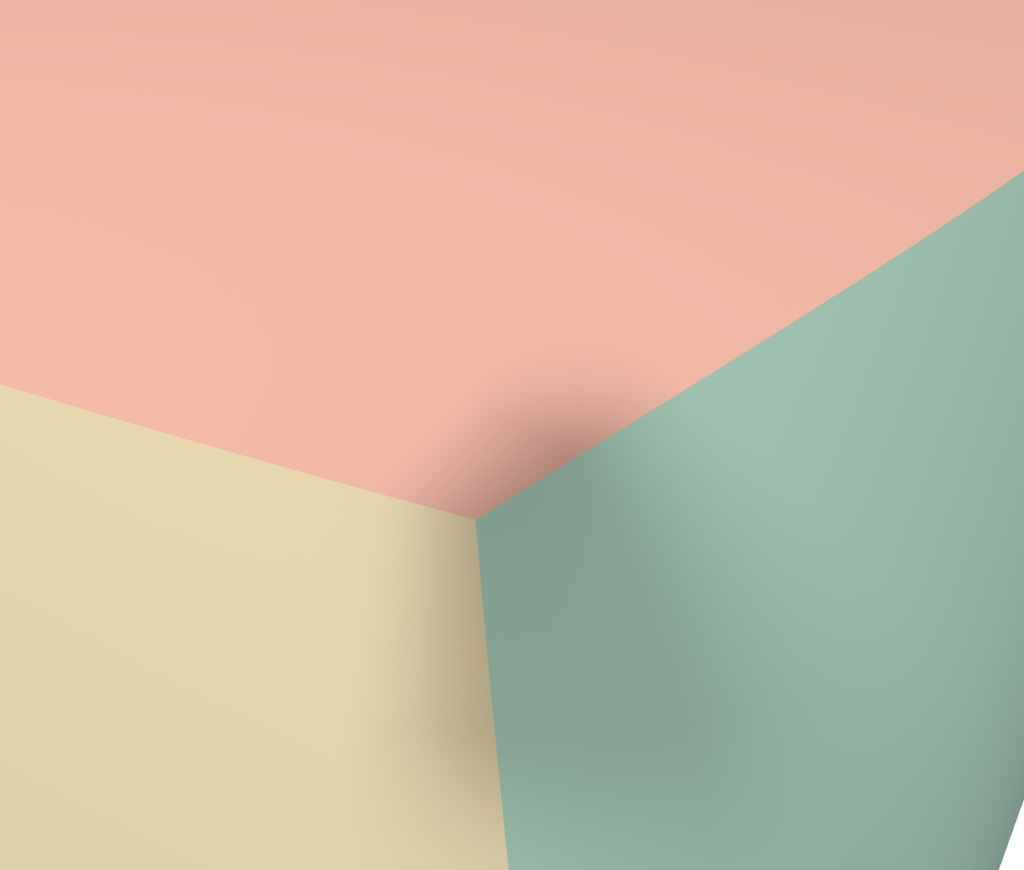
\includegraphics[width=\imagewidth]{pseudo_EdS_sommet/base_shadow}};
		%
		\foreach \iface in {1,...,\nfaces}
		{%
			\DTLassign{dbpointlabel}{\iface}{\px=x, \py=y, \pl=l}%
			\coordinate (p\iface) at ($(\px,\py)$);
			\pgfmathtruncatemacro\iq{\nfaces+\iface}
			\DTLassign{dbpointlabel}{\iq}{\qx=x, \qy=y, \ql=l}%
			\coordinate (q\iface) at ($(\qx,\qy)$);
		}%
		%
		\DTLassign{dbpointlabel}{\DTLrowcount{dbpointlabel}}{\clx=x, \cly=y, \clxl=xl, \clyl=yl, \cll=l}%
		\coordinate (c) at (\clx, \cly);
		{\transparent{0.72}%
			\node[img] at (0,0) {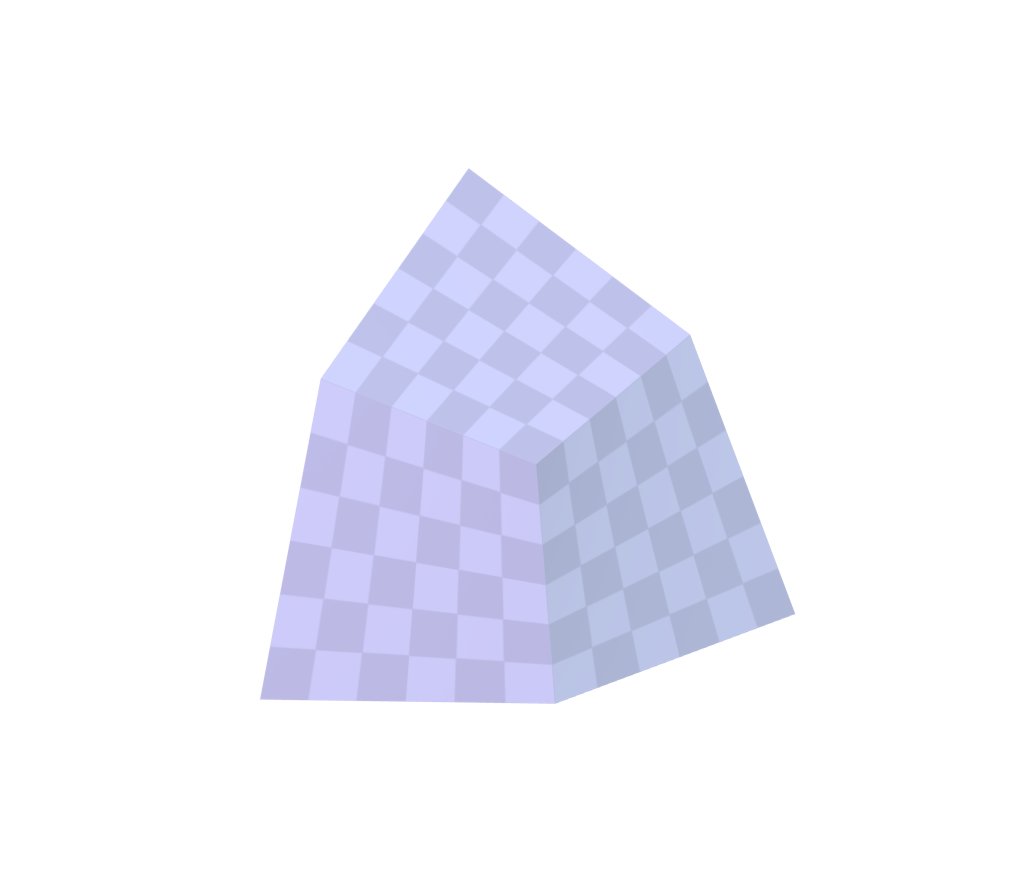
\includegraphics[width=\imagewidth]{pseudo_EdS_sommet/bilinear_only}};
		}%
		%
		\foreach \iface in {1,...,\nfaces}
		{%
			\pgfmathtruncatemacro\iiface{\iface - 1}
			{\transparent{0.8}%
				\draw[
					curv,
					dash pattern=on 2pt off 3pt,
				] plot file {figures/data/pseudo_EdS_sommet/quadpoly/xy_edge_hid_\iface.dat};
			}%
			\draw[
				curv,
				shorten >= 0.4pt,
				insert node={\node[label] {$\brepedge_{\iiface}$};} at 0.75 raised -1.8ex,
			] plot file {figures/data/pseudo_EdS_sommet/quadpoly/xy_edge_vis_\iface.dat};
			%
			\DTLassign{dbcolors}{\iface}{\fcolorr=r, \fcolorg=g, \fcolorb=b}%
			\definecolor{facecolor}{rgb}{\fcolorr, \fcolorg, \fcolorb}
			\ifnum \iface=1\relax%
				\colorlet{labelcolor}{facecolor!50!black}
				\raisevalue=1.7ex
			\else%
				\colorlet{labelcolor}{facecolor!60!black}
				\raisevalue=-1.7ex
			\fi%
			%
			\coordinate (n\iface) at (p\iface);%($(\vx, \vy)!0.5!(p\iface)$);
			\draw[vector, labelcolor] (\vx, \vy) -- (n\iface);
			%\draw[thick, dotted, labelcolor, shorten <= 1pt] (n\iface) -- (p\iface);
%			\path[
%				insert node={\node[labelcolor, labelpoint] {$\unv_{\iface}$};} at 0.49 raised -1.7ex,%\raisevalue,
%			] (\vx, \vy) -- (p\iface);
			\node[labelcolor, labelpoint] at ($(\vx, \vy)!1.12!(p\iface)$) {$\unv_{\iiface}$};
			%
			\pgfmathtruncatemacro\jface{1 + mod(\iface, \nfaces)}%
			\draw[thin, quadcolordark]
				(p\iface) -- (q\iface)
				(q\iface) -- (p\jface)
				      (c) -- (q\iface);
		}%
		%
		\DTLforeach{dbpointlabel}{\plx=x, \ply=y, \plxl=xl, \plyl=yl, \pll=l}%
		{%
			\fill[quadcolordark] (\plx, \ply) circle (1.2pt);
			\ifnum \arabic{DTLrowi}>\nfaces\relax%
				\node[quadcolordark, labelpoint] at (\plxl, \plyl) {$\pll$};
			\fi
		}%
		%
		%\drawGrid{10}{10}{thin, dotted};
		{\transparent{0.55}%
			\node[label] at (0.90, 0.45) {$\brepface_0$};
			\node[label] at (0.17, 0.85) {$\brepface_1$};
			\node[label] at (0.10, 0.30) {$\brepface_2$};
		}%
		%
		\fill[black] (\vx, \vy) circle (1.2pt);
		\node[above left, labelpoint] at (\vx, \vy) {$\v$};
		%
	\end{scope}
	%
	\begin{scope}[
		shift={(\textwidth-\imagewidth,0)}
	]
		%
		\node[img] at (0,0) {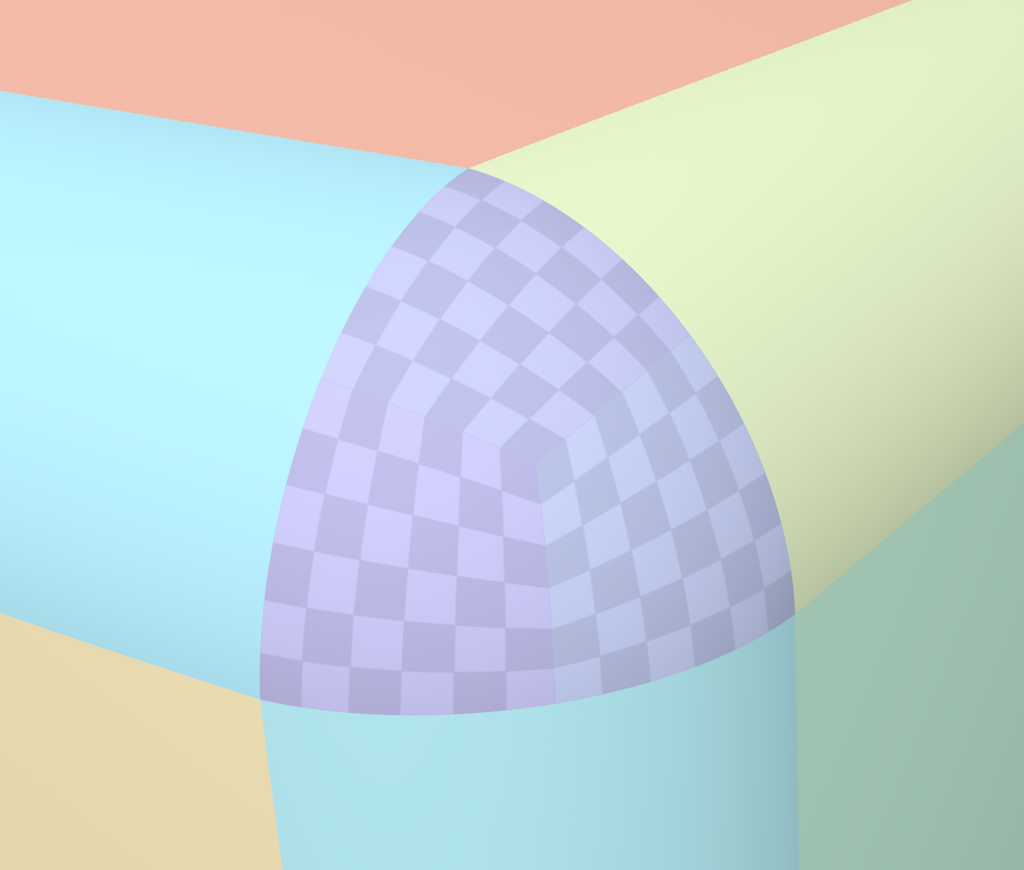
\includegraphics[width=\imagewidth]{pseudo_EdS_sommet/quadpoly}};
		%
		\DTLforeach{dbquadlabel}{\qlx=x, \qly=y}%
		{%
			\pgfmathtruncatemacro\iface{\arabic{DTLrowi}}%
			\pgfmathtruncatemacro\iiface{\iface - 1}%
			\pgfmathtruncatemacro\kface{1 + mod(\iface +  \nfaces - 2, \nfaces)}%
			\pgfmathtruncatemacro\kkface{\kface - 1}%
			\draw[
				curv,
				insert node={\node[label] {$\Gamma_{\kkface,\iiface}$};} at 0.25 raised -2ex,
				insert node={\node[label] {$\Gamma_{\iiface,\iiface}$};} at 0.75 raised -2ex,
			] plot file {figures/data/pseudo_EdS_sommet/quadpoly/xy_arc_\iface.dat};
			\draw[
				curv, 
				shorten >= 0.4pt,
				insert node={\node[label] {$\Gamma_{\iiface}$};} at 0.5 raised -1.5ex,
			] plot file {figures/data/pseudo_EdS_sommet/quadpoly/xy_quadsep_\iface.dat};
			%
			{\transparent{0.55}%
				\node[label] at (\qlx, \qly) {$\pseudoEdS{\brepvertex}{\rho}[\iiface]$};
			}%
		}%
		%
%		\DTLforeach{dbpointlabel}{\plx=x, \ply=y, \plxl=xl, \plyl=yl, \pll=l}%
%		{%
%			\fill[black] (\plx, \ply) circle (1.2pt);
%			\node[labelpoint] at (\plxl, \plyl) {$\pll$};
%		}%
		%
		%\drawGrid{10}{10}{thin, dotted};
		{\transparent{0.55}%
			\node[label] at (0.90, 0.20) {$\EdSpropreplus{\brepface_0}{\rho}$};
			\node[label] at (0.45, 0.92) {$\EdSpropreplus{\brepface_1}{\rho}$};
			\node[label] at (0.13, 0.10) {$\EdSpropreplus{\brepface_2}{\rho}$};
			%
			\node[label] at (0.55, 0.05) {$\pseudoEdS{\brepedge_0}{\rho}$};
			\node[label] at (0.85, 0.74) {$\pseudoEdS{\brepedge_1}{\rho}$};
			\node[label] at (0.13, 0.58) {$\pseudoEdS{\brepedge_2}{\rho}$};
		}%
	\end{scope}
	%
	\end{tikzpicture}
	\DTLgdeletedb{dbvertex}%
	\DTLgdeletedb{dbquadlabel}%
	\DTLgdeletedb{dbpointlabel}%
	\DTLgdeletedb{dbcolors}%
	%
	\caption{Représentation de la pseudo-EdS d'un sommet à l'aide de plusieurs carreaux non-restreints.}
	\label{fig:pseudo_EdS_sommet_quadpoly}
\end{figure}




avantages/inconvénients :
\begin{itemize}
	\item[$-$] valable seulement si la vitesse normale est uniforme
	\item[$-$] génère plusieurs nouveaux carreaux de surface
	%\item[$+$] les nouveaux carreaux sont rectangulaires ($\Rightarrow$ permet l'utilisation de quadratures simples (\cf \autoref{section:clenshaw_curtis_quadrature})
	\item[$+$] utiliser des carreaux paramétriques non restreints présente plusieurs avantages :
	\begin{enumerate}
		\item permet l'utilisation de quadratures simples (\cf \autoref{section:clenshaw_curtis_quadrature})
		\item simplifie les tests de sortie du domaine paramétrique (\cf partie optimisation de maillage trans-carreaux)
	\end{enumerate}
\end{itemize}


\subsubsection{Ajustement d'un seul carreau restreint}%Ajustement de carreau sphérique à un nuage de points}
\label{section:ajustement_carreau_spherique}
\def\s{\vit{s}}
On suppose maintenant que $\rho$ peut varier continument sur $\Sigma$. 

\begin{enumerate}
	\item on cherche alors à construire un seul carreau paramétrique restreint qui contient les arcs de cercles caractéristiques aux extrémités des arêtes \brep\ incidentes à $\brepvertex$
	\item afin de simplifier la construction, on considère que $\v$ est situé à l'origine et que $\rho(\v) = 1$ (on appliquera la transformation adéquate en fin de construction pour se placer à nouveau dans le cas général)
	\item le problème consiste alors, étant donné un ensemble $C$ de courbes sur la sphère unité $\mathbb{S}^2$, à construire un carreau paramétrique décrivant une région $\Sigma_S$ de $\mathbb{S}^2$ contenant $C$
	\item on cherche également à faire en sorte $\Sigma_S$ englobe $S$ le plus étroitement possible ($\sim$ minimisation de l'aire) \textit{(développer motivation\ldots)}
	
	\item on choisit d'utiliser les coordonnées sphériques comme paramètres, \ie
	\begin{equation}
	    \bs = \mathbf{R} 
	    \begin{pmatrix}
		    \cos \theta \cos \lambda \\
		    \sin \theta \cos \lambda \\
		    \sin \lambda \\
	    \end{pmatrix},
	\end{equation}
	où $\mathbf{R}$ désigne une matrice de rotation (\ie ses colonnes forment une base orthonormée de $\reals^3$) et $\theta$, $\lambda$ désignent respectivement la longitude et la latitude d'un point du carreau
	\begin{align*}
	    \theta(u,v)  &= \Theta u + \theta_0, \\
	    \lambda(u,v) &= \Lambda v + \lambda_0,
	\end{align*}
	avec $-1 \leq u, v \leq 1$


	\item on propose donc une méthode heuristique pour construire un tel carreau (\ie trouver $\mathbf{R}$, $\Theta$, $\theta_0$, $\Lambda$ et $\lambda_0$) d'aire minimale
	\item on suppose qu'on dispose d'un échantillonnage suffisamment $S = \family{\s}{i}{1}{n}$ fin de l'ensemble des arcs de cercle caractéristiques limites
	\item le problème consiste alors à construire un carreau paramétrique décrivant une région $\Sigma_S$ de $\mathbb{S}^2$ contenant $S$
	
	\item On note $\s_{0} = \sum_{i = 1}^n \s_i$. 
	On suppose pour le moment que $\normtwo{\s_{0}} \neq 0$. 
	On définit alors 
	\begin{equation}
	    \vrm{r}_1 = \unitized{ \s_{0} }.
	\end{equation}
\end{enumerate}	

%(\cf notes Huygens)
avantages/inconvénients :
\begin{itemize}
	\item[$-$] le nouveau carreau est restreint
	\item[$+$] valable également si la vitesse normale varie spatialement
	\item[$+$] génère un seul nouveau carreau de surface
\end{itemize}

%%Soit $\brepvertex$ un sommet \brep\ convexe dont le support géométrique est le point $\v \in \reals^3$. 
%%On cherche à construire un carreau paramétrique restreint décrivant $\pseudoEdS{\v}{\rho}$ \ie la région de la sphère $\sphere[\v][\rho(\v)]$ délimitée par les arcs de cercles caractéristiques aux extrémités des arêtes \brep\ incidentes à $\v$. 
%Afin de simplifier cette construction, on considère que $\v$ est situé à l'origine et que $\rho(\v) = 1$. 
%(On appliquera la transformation adéquate en fin de construction pour se placer à nouveau dans le cas général.)
%\par
%Le problème consiste alors, étant donné un ensemble de points $S = \family{\s}{i}{1}{n}$ sur la sphère unité $\mathbb{S}^2$, à construire un carreau paramétrique décrivant une portion $R$ de $\mathbb{S}^2$ contenant $S$. 
%On cherche également à minimiser l'aire de $R$ \ldots




\section{Construction d'un modèle \brep\ de l'EdB}

\subsection{Construction du graphe des intersections}
Conservation/création des intersections tangentielles, calcul des intersections transverses entre paire de carreaux non-restreints, segmentation des courbes d'intersection en segments quasi-disjoints (intersection de 3 carreaux non-restreints ou plus), \guillemets{clipping} par le domaine paramétrique de chaque carreau restreint
\par\bigskip
pour un carreau de surface, il s'agit d'un graphe planaire orienté dont un plongement dans $\reals^2$ est donné par la trace des courbes d'intersections dans son espace paramétrique

\begin{figure}
	\centering
	\plotCurvedDirectedGraph{/d/bandrieu/GitHub/FFTsurf/test/graph/graph_bezier_control_points.dat}{25mm}
	\caption{Plongement du graphe des intersections dans l'espace paramétrique d'un carreau de surface.}
\end{figure}


\subsection{Construction des faces, arêtes et sommets \brep}
pour chaque carreau : extraction des cycles du graphe d'intersection, caractérisations des contours (extérieurs/intérieurs), détermination des faces $\to$ insertion des contours dans la \brep\ $\to$ insertion des (co-)arêtes et sommets
\begin{figure}
	\centering
	\newcommand{\arc}{\mathcal{A}}%
\newcommand{\subin}{\ensuremath{_{\mathrm{in}}}}%
\newcommand{\subout}{\ensuremath{_{\mathrm{out}}}}%
\newcommand{\noeud}{\mathcal{N}}%
\newcommand{\cycle}{\mathcal{C}}%
\newcommand{\graph}{\mathcal{G}}%
\begin{tikzpicture}[%
	scale=0.5,
	>={Latex[length=4pt]},      % Arrow style
    start chain=going below,    % General flow is top-to-bottom
    node distance=6mm and 50mm, % Global setup of box spacing
    every join/.style={flow},   % Default linetype for connecting boxes
    ]
% ------------------------------------------------- 
% A few box styles 
% <on chain> *and* <on grid> reduce the need for manual relative
% positioning of nodes
\tikzset{
  base/.style={draw, on chain, on grid, align=center, minimum height=4ex, minimum width=5em},
  proc/.style={base, rectangle},
  test/.style={base, diamond, aspect=2},
  term/.style={proc, rounded corners=2ex},
  % coord node style is used for placing corners of connecting lines
  coord/.style={coordinate, on chain, on grid, node distance=6mm and 25mm},
  % -------------------------------------------------
  % Connector line styles for different parts of the diagram
  flow/.style={->, draw}
}
% -------------------------------------------------
\node [term, join] (start) {Début};
\node [proc, join] (p1) {Éliminer les branches pendantes de $\graph$};
\node [test, join] (t1) {$A = \emptyset$ ?};

\node [proc] (startarc) {Choisir un arc $\arc_*$ de $\graph$};

\node [proc, join] {Démarrer un nouveau cycle $\cycle$ à partir de $\arc_*$};
\node [proc, join] {$\arc \leftarrow \arc_*$ et\\ $\noeud \leftarrow \dest(\arc)$};


\node [test, join] (t2) {$\noeud = \orig(\arc_*)$?};

\node [proc] (maxangles) {Identifier $\hi{\alpha}\subin$, $\hi{\alpha}\subout$ et $\hi{\arc}\subout$};


\node [test, join] (t3) {$\hi{\alpha}\subin > \hi{\alpha}\subout$ ?};
\node [proc] (abortcycle) {Abandonner $\cycle$};

\node [term, left=of t1, text width=3em] (end) {Fin};
\node [proc, right=of t2] (completecycle) {Rajouter $\cycle$\\à la liste des cycles\\et l'extraire de $\graph$};
\node [proc, left=of t3] (appendcycle) {$\arc \leftarrow \hi{\arc}\subout$,\\ $\noeud \leftarrow \dest(\arc)$ et \\ajouter $\arc$ à $\cycle$};


\draw [flow] (t1.west) -- node[above] {oui} (end);
\draw [flow] (t1.south) -- node[left] {non} (startarc);

\draw [flow] (t2.east) -- node[above] {oui} (completecycle);
\draw [flow] (t2.south) -- node[left] {non} (maxangles);

\draw [flow] (t3.west) -- node[above] {oui} (appendcycle);
\draw [flow] (t3.south) -- node[left] {non} (abortcycle);


\draw [flow] (appendcycle.north) |- (t2);

\node [coord, left=of appendcycle] (c2)  {};
\draw [flow] (abortcycle.west) -| (c2) |- (p1);

\draw [flow] (completecycle.north) |- (p1);
% -------------------------------------------------
\end{tikzpicture}
	\caption{Organigramme de l'algorithme d'extraction des cycles d'un graphe orienté plongé dans $\reals^2$.}
\end{figure}


\begin{figure}
	\centering
	\setlength{\imagewidth}{60mm}%
\setlength{\imageheight}{\imagewidth}%
%
\colorlet{facecolor1}{mycolor_1}
\colorlet{facecolor2}{mycolor_2}
\colorlet{facecolor3}{mycolor_3}
%
\begin{tikzpicture}[
	x=0.5\imagewidth, 
	y=0.5\imageheight,
	halfedge/.style={
		line width=0.8pt, 
		line cap=round, 
		-{Triangle[left]}
	},
]
	%\input{/d/bandrieu/GitHub/FFTsurf/test/graph/graph_faces_tikzcode.tex}
	\input{../../FFTsurf/test/graph/graph_faces_tikzcode.tex}
\end{tikzpicture}

	\caption{Faces du graphe}
\end{figure}